\documentclass[11pt,a4paper,oneside]{report}

% ============================================================
% PACKAGES
% ============================================================

\usepackage[utf8]{inputenc}
\usepackage[T1]{fontenc}
\usepackage[french]{babel}
\usepackage{csquotes}
\usepackage{tabularx} 
\usepackage{subcaption} 
\usepackage{array}
\usepackage{multirow}
\usepackage{booktabs}
\usepackage{lmodern}
\usepackage{microtype}
\usepackage{amsmath}
\usepackage{dsfont}

% Mise en page — marges resserrées
\usepackage[
a4paper,
top=2cm,
bottom=2cm,
left=2.5cm,
right=2cm
]{geometry}

% Maths
\usepackage{amsmath,amssymb,amsfonts}

% Figures
\usepackage{graphicx}
\usepackage{float}

% Tableaux
\usepackage{longtable}

% Légendes — espacement réduit avant/après
\usepackage[
font=small,
labelfont=bf,
justification=centering,
skip=4pt
]{caption}

% Références
\usepackage[
backend=biber,
style=numeric-comp,
sorting=none
]{biblatex}

\addbibresource{references.bib}

% Liens
\usepackage[
colorlinks=true,
linkcolor=black,
citecolor=black,
urlcolor=black
]{hyperref}

% Espacement — interligne resserré au lieu de 1.5
\usepackage{setspace}
\singlespacing
% Si single est trop serré à ton goût, remplace par :
% \setstretch{1.1}

% Espacement des paragraphes (au lieu du \parskip par défaut si tu en ajoutes un ailleurs)
\setlength{\parskip}{0pt}
\setlength{\parindent}{1.2em}

% Espacement des listes (itemize/enumerate) plus compact
\usepackage{enumitem}
\setlist{itemsep=2pt, topsep=4pt, parsep=0pt}

% En-têtes / pieds de page
\usepackage{fancyhdr}

% ============================================================
% PAGE STYLE
% ============================================================

\pagestyle{fancy}
\fancyhf{}

\fancyhead[L]{\small \leftmark}
\fancyhead[R]{\small \thepage}
\fancyfoot[C]{\small NICOLAS Elise}

\renewcommand{\headrulewidth}{0.4pt}
\renewcommand{\footrulewidth}{0pt}

\fancypagestyle{plain}{
	\fancyhf{}
	\fancyfoot[C]{\small NICOLAS Elise}
	\renewcommand{\headrulewidth}{0pt}
}

% ============================================================
% STYLE DES TITRES — espacements réduits
% ============================================================

\usepackage{titlesec}

% Part
\titleformat{\part}
{\normalfont\Huge\bfseries}
{Part \thepart}
{1em}{}

% Chapter — espace après très réduit (30pt -> 12pt)
\titleformat{\chapter}
{\normalfont\huge\bfseries}
{\thechapter}
{1em}{}

\titlespacing*{\chapter}
{0pt}{-20pt}{12pt}

% Sections — espacement avant/après resserré
\titleformat{\section}
{\normalfont\Large\bfseries}
{\thesection}
{1em}{}

\titlespacing*{\section}
{0pt}{2.5ex plus 1ex minus .2ex}{1ex plus .2ex}

% Sous-sections
\titleformat{\subsection}
{\normalfont\large\bfseries}
{\thesubsection}
{1em}{}

\titlespacing*{\subsection}
{0pt}{2ex plus 1ex minus .2ex}{0.8ex plus .2ex}

% Sous-sous-sections
\titleformat{\subsubsection}
{\normalfont\normalsize\bfseries}
{\thesubsubsection}
{1em}{}

\titlespacing*{\subsubsection}
{0pt}{1.5ex plus 1ex minus .2ex}{0.5ex plus .2ex}

\titleformat{\paragraph}
{\normalfont\normalsize\bfseries}
{\theparagraph}
{1em}{}

\titlespacing*{\paragraph}
{0pt}{1.5ex plus 1ex minus .2ex}{0.5ex plus .2ex}

\setcounter{secnumdepth}{3}

\usepackage{pdflscape}
\begin{document}
	\begin{titlepage}
		\centering
		
		% ============================================================
		% BANDEAU DE LOGOS
		% ============================================================
		\vspace*{0.3cm}
		
		\noindent
		\begin{minipage}[c]{0.24\textwidth}
			\centering
			
\includegraphics[width=\textwidth]{images/00_logos/UniversiteParisCite_logo_horizontal_couleur_CMJN}
		\end{minipage}%
		\hfill
		\begin{minipage}[c]{0.22\textwidth}
			\centering
			
\includegraphics[width=0.85\textwidth]{images/00_logos/Logo_MIO-eng}
		\end{minipage}%
		\hfill
		\begin{minipage}[c]{0.22\textwidth}
			\centering
			
\includegraphics[width=0.85\textwidth]{images/00_logos/logo_CEBC_PJG_24-300x164}
		\end{minipage}%
		\hfill
		\begin{minipage}[c]{0.22\textwidth}
			\centering
			
\includegraphics[width=0.85\textwidth]{images/00_logos/logo_locean_1}
		\end{minipage}
		
		\vspace{1.4cm}
		
		% ============================================================
		% UNIVERSITÉ ET FORMATION
		% ============================================================
		{\scshape\LARGE Université Paris Cité\par}
		
		\vspace{0.35cm}
		
		{\large
			Master 2 Mathématiques et Informatique Appliquées à la Science des Données
			\par}
		
		\vspace{1.15cm}
		
		% ============================================================
		% TITRE
		% ============================================================
		{\Large\bfseries
			Modélisation de la relation entre structuration environnementale,
			communautés phytoplanctoniques et distribution des Niveaux
			Trophiques Intermédiaires
			\par}
		
		\vspace{0.25cm}
		
		{\large
			Une étude en saison estivale dans le secteur Indien de l'Océan Austral
			\par}
		
		\vspace{0.25cm}
		
		{\large
			Rapport de stage
			\par}
		
		\vfill
		
		% ============================================================
		% AUTEUR
		% ============================================================
		{\large\bfseries Rapport réalisé par\par}
		\vspace{0.15cm}
		{\large Elise NICOLAS\par}
		
		\vspace{0.55cm}
		
		% ============================================================
		% ENCADRANTS
		% ============================================================
		{\large\bfseries Encadrants\par}
		\vspace{0.15cm}
		{\large
			Marius MOLINET, David NERINI, Christophe GUINET, Cédric COTTE
			\par}
		
		\vspace{0.55cm}
		
		% ============================================================
		% PROFESSEURE RÉFÉRENTE
		% ============================================================
		{\large\bfseries Professeure référente\par}
		\vspace{0.15cm}
		{\large Aurélie FISHER\par}
		
		\vspace{0.55cm}
		
		% ============================================================
		% DATE
		% ============================================================
		{\large Septembre 2026\par}
		
		\vspace*{0.4cm}
		
	\end{titlepage}
	
	%------------------------------------
	\clearpage
	\begin{abstract}
	
	\textbf{Contexte.} Le réchauffement climatique modifie la structure des communautés phytoplanctoniques de l'océan Austral, avec une possible diminution de la contribution des diatomées au profit du nano- et picophytoplancton. Ce changement pourrait allonger le réseau trophique et affecter la biomasse des Niveaux Trophiques Intermédiaires (NTI, zooplancton et micronecton), avec des répercussions en cascade sur l'ensemble des écosystèmes.
	
	\vspace{0.3cm}
	
	\textbf{Objectif et méthode.} La relation entre la biomasse des NTI, estimée par acoustique active (Nautical Area Scattering Coefficient, NASC, à 38 et 120 kHz) a été modélisée avec des Forêts aléatoires par un ensemble de variables environnementales (température, salinité, hydrodynamisme via le Finite-Time Lyapunov Exponent) et pigmentaires (neuf pigments photosynthétiques). L'étude porte sur le secteur indien de l'océan Austral, en saison estivale (janvier-mars), à partir des campagnes OBSAUSTRAL 2018, 2021, 2022 et 2023. Une attention particulière a été portée à la fiabilité de l'évaluation et l'interprétation du modèle : une comparaison entre validation croisée Monte-Carlo et validation par blocage spatio-temporel a été effectuée. 
	%Des communautés phytoplanctoniques de la région ont ensuite été caractérisées par clustering k-means sur les concentrations pigmentaires. 
	
	\vspace{0.3cm}
	
	\textbf{Résultats.} Des cartes de prédictions de NASC ont été générées sur l'ensemble de la région pour chaque modèle de validation croisée. Malgré des écarts de performance importants entre les schémas de validation, les cartes obtenues sont similaires. Elles révèlent une structuration latitudinale inversée entre 38 et 120 kHz. Les domaines océanographiques fonctionnels (température/salinité) et la biomasse phytoplanctonique totale ressortent comme les plus importantes variables pour la prédiction du NASC et le microphytoplancton (diatomées, dinoflagellés) apparaît plus déterminant que le nano- et le picophytoplancton. La comparaison entre validation croisée Monte-Carlo et validation par blocage spatio-temporel révèle une fuite d'information substantielle dans le premier schéma, confirmée par une forte sensibilité au bruit.  Chaque schéma de validation témoigne d'un plafond structurel des courbes d'apprentissage dont l'origine, limite informationnelle des covariables, densité d'échantillonnage, ou non-stationnarité spatiale non prise en compte, n'a pu être totalement départagée. 
	%Une seconde analyse par clustering des concentrations pigmentaires met en évidence six communautés phytoplanctoniques structurées selon un gradient latitudinal sans toutefois révéler de différence significative de NASC entre ces communautés. 
	
	
	\vspace{0.3cm}
	
	\textbf{Conclusion et perspectives.} Ces résultats suggèrent que la structuration environnementale (physico-chimique et hydrodynamique) prédomine sur la seule composition pigmentaire dans l'explication de la distribution du NASC par le Random Forest, sur la période et l'échelle considérées. Ils soulignent également la nécessité d'une évaluation méthodologiquement rigoureuse dans les modèles écologiques spatio-temporels. Des travaux futurs pourraient intégrer une méthode de sélection de variable plus étoffée, la complétion de données manquantes, un décalage temporel entre efflorescence phytoplanctonique et réponse des NTI, l'intégration explicite de la non-stationnarité, l'exploitation de données de bio-logging pour élargir la couverture spatio-temporelle, et recourir à des modèles de machine learning causal pour identifier les relations biologiques entre les variables étudiées.
	
	\vspace{0.5cm}
	\noindent\textbf{Mots-clés :} océan Austral, niveaux trophiques intermédiaires, acoustique active, phytoplancton, arbres de régression, validation croisée spatio-temporelle
\end{abstract}
	
	%------------------------------------
	%------------------------------------
	\clearpage
	\tableofcontents
	
	%------------------------------------
	% Chapitres 
	\clearpage
	\chapter{Introduction}

Le phytoplancton désigne l'ensemble des organismes unicellulaires photosynthétiques (« phyto ») dépourvus de capacité de déplacement autonome contre le courant (« plancton »). Ces organismes soutiennent les écosystèmes marins en constituant le premier maillon de la chaîne alimentaire, aussi appelée réseau trophique. Ils jouent par ailleurs un rôle fondamental dans le cycle du carbone, en structurant, par leur taille, leur composition et leur abondance, les apports de carbone vers les fonds marins. On parle de communauté phytoplanctonique pour désigner un assemblage particulier d'organismes phytoplanctoniques dans un espace et à un temps donné \cite{reynolds2006ecology}.

\vspace{0.3cm}

Le réchauffement climatique induit des changements rapides dans l'océan Austral : l'eau se réchauffe et s'adoucit sous l'effet de la fonte des glaces, les champs de courants et de vents se modifient, la stratification de la colonne d'eau s'accentue, etc. \cite{sallee2018} \cite{abram2025Antarctic}. Ces changements ne sont pas sans conséquences pour les communautés phytoplanctoniques \cite{deppeler2017southern}. Des études récentes montrent des changements de phénologie \cite{thomalla2023Widespread}\cite{boyce2017environmental}, d'abondance \cite{hayward2024Antarctic} et de structuration des communautés phytoplanctoniques \cite{adroli2026}.

\vspace{0.3cm}

Dans l'océan Austral, ces communautés sont dominées par les diatomées, larges cellules phytoplanctoniques (microphytoplancton, 20-200 $\mu m$) à forte valeur énergétique \cite{treguer1992} \cite{heidemann2024drivers}. Les modifications induites par le réchauffement climatique tendraient à augmenter la biomasse phytoplanctonique \cite{delcastillo2019greener} \cite{adroli2026} tout en diminuant la contribution relative des diatomées au profit du nano- et picophytoplancton, organismes à plus faible valeur énergétique \cite{krumhardt2022climate}\cite{sari2025influence}. Les diatomées soutiennent un réseau trophique court et hautement productif \cite{treguer1992}. Elles sont consommées par le grand zooplancton (copépodes, krill) et le micronecton (petits poissons), regroupés sous l'appellation de Niveaux Trophiques Intermédiaires (NTI). Ces organismes sont eux-mêmes consommés par de plus gros poissons pélagiques, à leur tour proies de plus grands prédateurs. Un changement de structuration des communautés phytoplanctoniques vers une plus forte proportion de petit phytoplancton favoriserait ainsi le développement d'un zooplancton de plus petite taille, lui-même consommé par des organismes plus petits \cite{krumhardt2022climate}. Ainsi, on observerait un allongement du réseau trophique et donc une modification du transfert d'énergie à chacun des ses maillons jusqu'aux prédateurs supérieurs \cite{mestre2020decadal} : on parle de cascade trophique. Un changement d'assemblage des communautés phytoplanctonique impacterait donc l'ensemble de l'écosystème.


\vspace{0.3cm}

Caractériser ces changements est par conséquent nécessaire, mais difficile dans les écosystèmes pélagiques \footnote{Ensemble des organismes et de leur environnement vivant dans la colonne d'eau du large, c'est-à-dire en pleine eau, loin du fond et des côtes, par opposition au domaine benthique lié au fond marin.} : ces milieux étant très vastes et peu accessibles, leur échantillonnage à grande échelle est logistiquement couteux. L'acoustique active constitue un moyen d'étude des NTI dans ces zones difficiles d'accès. Elle consiste à émettre une onde, à la réceptionner, puis à analyser le signal reçu (principe du sonar) \cite{benoitbird2016ecological}. L'écho reçu résulte de la réflexion du son émis sur un objet (le fond marin, par exemple), un organisme, ou encore une discontinuité physique dans la colonne d'eau (changement de densité). La connaissance de la vitesse locale de propagation du son dans l'eau permet, à partir du délai de réception du signal et de son intensité, de renseigner la profondeur, l'abondance et d'inférer sur la composition taxonomique des organismes présents \cite{benoitbird2016ecological}. Le Nautical Area Scattering Coefficient (NASC), calculé à partir des échos acoustiques reçus, permet de résumer la rétrodiffusion acoustique sur un ensemble de profondeur considérées en un certain point de l'espace \cite{maclennan2002}. Il sert donc de proxy de la biomasse de NTI à cette localisation. L'océan Austral étant particulièrement vaste et difficile d'accès, les campagnes d'échantillonnages restent limitées et, dans ce contexte, il est particulièrement pertinent de développer des modèles prédictifs permettant de généraliser les estimations faites à partir des données déjà acquises.

\vspace{0.3cm}

Cette étude à cherché à développer un modèle prédictif de la biomasse des NTI en fonction de l'assemblage des communautés phytoplanctoniques et de l'activité de mésoéchelle. Plus précisément, nous avons modélisé le NASC avec des Forêts Aléatoires en fonction de 9 variables de concentration pigmentaires ($P_1, P_2, \ldots, P_9$), 2 variables physique, la température et salinité (FOD), et 1 variable capturant l'hydrodynamisme (FTLE). Ainsi, nous avons cherché à documenter la relation $NASC \sim FTLE + FOD + P_1 + P_2 + \ldots + P_9$. Ce modèle, développé sur le secteur indien de l'océan Austral à partir de données d'acoustique active collectées lors des campagnes OBSAUSTRAL 2018, 2021, 2022 et 2023, à permis de créer des cartes prédictives de NASC sur l'ensemble de la région et de mettre en évidence les variables environnementales clés pour la prédiction. L'objectif étant d'informer les conséquences de la restructuration des communautés phytoplanctoniques sur les NTI du secteur Indien de l'océan Austral.

\vspace{0.3cm}

La section \textbf{Matériel} détaillera la nature des données utilisées (acoustique active, température, salinité, champs de courants et concentrations pigmentaires). La section \textbf{Méthode} présentera le calcul des variables d'intérêt NASC, FTLE et FOD. Cette section décrira ensuite brièvement la méthode Random Forest, le calcul de l'importance des variables et le pipeline d'apprentissage mis en place. La section \textbf{Résultat} présentera (1) les cartes de NASC prédites (2) les variables environnementales identifiées comme importantes pour la prédiction du NASC (3) l'interprétation du modèle. La \textbf{Discussion }portera sur la fiabilité du modèle, la difficultée liée à la nature même des données et la mise en perspective avec la littérature de l'effet structurant des variables environnementales considérées et de la nature des communautés phytoplanctoniques.

	\clearpage
	\chapter{Matériel et pré-traitement des données }% construction des métriques
La biomasse de zooplancton et micronecton, l'assemblage des communautés phytoplanctoniques, l'environnement physique des organismes ne sont pas directement mesurables, ce sont des construits (\textit{constructs}), c'est à dire des abstractions qui décrivent le phénomène théorique d'intérêt \cite{edwards2000nature}. Pour étudier ces phénomènes, nous avons besoin de trouver des variables mesurables pouvant les décrire, c'est l'opérationnalisation du construit. Les choix des variables utilisées sont justifiées par la connaissances théorique des phénomènes étudiés, appuyés par la littérature. Les variables mesurables sont alors dites variables \textit{proxy} pour les construits associés. \cite{shmueli2010explain}.
 
 
 Les variables proxy sélectionnées sont les suivantes : (1) le Nautical Area Scattering Coefficient(NASC) approxime la biomasse du zooplancton et micronecton sur l'ensemble de la profondeur considérée; (2) les concentrations pigmentaires ($P_1, \ldots, P_9$) approximent l'assemblage des communautés phytoplanctoniques leur abondance totale; (3) le Finite-Time Lyapunov Exponent (FTLE) approxime l'hydrodynamisme et (4) la température et la salinité rendent compte des conditions physico-chimiques du milieu.
 
 Toutes les données utilisées pour cette étude sont des données secondaires, c'est-à-dire que le plan d'échantillonnage n'a pas été construit spécifiquement pour répondre à cette problématique.
 
 \section{Zone d'étude et plan d'échantillonnage}
 
 L'étude a été réalisée sur les années 2018, 2021, 2022 et 2023, en saison estivale (janvier-mars) afin de limiter la variabilité saisonnière, et de jour (calculé selon l'angle solaire), afin de limiter l'effet de la migration verticale journalière (DVM) \footnote{Déplacement synchronisé dans la colonne d'eau au rythme du cycle jour/nuit : les organismes résident en profondeur durant le jour et remontent vers la surface la nuit, principalement pour se nourrir tout en réduisant le risque de prédation visuelle en eaux éclairées. Ce phénomène est considéré comme le plus grand mouvement synchronisé de biomasse à l'échelle de la planète. \cite{Bandara2021}}. La fenêtre d'étude a été fixée à [45,90]°E de longitude et [30, 60]°S de latitude afin de cibler précisémment le secteur indien de l'Océan Austral.
 
 \section{Données d'acoustique active (OBSAUSTRAL) et construction du Nautical Area Scattering Coefficient (NASC)}
 
 \subsection{Données d'acoustique active}
 Les données d'acoustiques actives ont été collectées par transects \footnote{Le bateau se déplace et collecte en même temps des données, par opposition aux données "stations" collectées lorsque le bateau est en arrêt. Cela a un coût en terme de résolution des spectrogramme et d'interprétabilité mais permet d'obtenir une plus grande couverture spatiale.} lors des campagnes océanographiques OBSAUSTRAL/THEMISTO 2018, 2021, 2022, 2023 en saison estivale. Ils sont détaillés sur la figure \ref{fig:transectsparannee2} \cite{flotteoceanographique_campagnes}.  
 \begin{figure}[H]
 	\centering
 	\includegraphics[width=0.6\textwidth]{images/02\_materiel\_et\_methode/active\_acoustic\_et\_NASC/transects\_par\_annee\_2}
 	\caption{Carte des transects effectués par le Marion Dufresnes II lors des campagnes océanographiques OBSAUSTRAL/THEMISTO 2018, 2021, 2022 et 2023.}
 	\label{fig:transectsparannee2}
 \end{figure}
 
 \vspace{1cm}
 
 Deux fréquences d'émissions ont été sélectionnées: 38 kHz, afin de comparer nos résultats avec la littérature \footnote{La méthode d'acoustique active ayant été développée par les pêcheries, la fréquence d'échosondeur de référence est 38kHz (fréquence à laquelle les poissons sont facilement détectables).} et 120 kHz, fréquence à laquelle les zooplanctons d’intérêts, Euphausiacés (krill) et Copépodes, sont les plus détectables (voir Annexe \ref{annexe:rep_freq}, figure \ref{fig:freqresponse}). Les échogrammes (figures \ref{fig:echogramme38khz2023-01-28} et \ref{fig:echogramme120khz2023-01-28}) donnent un aperçu de la nature des données collectées et de la manière dont l'information contenue par le signal reçu (résolution, organismes visibles) est déterminée par la fréquence de l'onde émise. Une forte intensité de l’écho reçu traduis la présence d'une importante biomasse d'organisme à ce temps, localisation géographique et profondeur.
 
 \begin{figure}[H]
 	\centering
 	\begin{subfigure}[t]{0.7\textwidth}
 		\centering
 		\includegraphics[width=\textwidth]{images/02\_materiel\_et\_methode/active\_acoustic\_et\_NASC/echogramme\_38kHz\_2023-01-28.png}
 		\caption{Fréquence d'émission de 38 kHz}
 		\label{fig:echogramme38khz2023-01-28}
 	\end{subfigure}
 	\vfill
 	\begin{subfigure}[t]{0.7\textwidth}
 		\centering
 		\includegraphics[width=\textwidth]{images/02\_materiel\_et\_methode/active\_acoustic\_et\_NASC/echogramme\_120kHz\_2023-01-28.png}
 		\caption{Fréquence d'émission de 120 kHz}
 		\label{fig:echogramme120khz2023-01-28}
 	\end{subfigure}
 	\caption{Exemple d'échogramme obtenu le 2023-01-28 entre 18h et 00h aux fréquences (a) 38 kHz et (b) 120 kHz}
 	\label{fig:echogramme2023-01-28}
 \end{figure}
 
 \subsection{Construction du Nautical Area Scattering Coefficient (NASC)}
 
	 L'\textbf{Intensité de l'echo (Echo Level EL) }correspond au signal reçu par le transducteur lorsqu'une onde est émise dans la colonne d'eau puis réfléchis par un objet.
	 \begin{equation}
	 	EL = SL - 2TL + DI + TS
	 \end{equation}	
	 où 
	 \begin{itemize}
	 	\item SL (Source Level): intensité du son émise (dB) $SL = 10 \times \log_{10}(I/I_{ref}) $ et $I_{ref} = \rho_{ref}^{2} = 1 \mu \text{Pa}$ ($\rho_{ref}$ la pression de référence)
	 	\item TL (Transmission Loss): perte de transmission  \footnote{Le premier terme correspond à l'attenuation due à la dispersion de l'onde et le second terme correspondant à l'éttenuation de la propagation du milieu ($\alpha$ le coefficient d'absorption en $dB.m^{-1}$)} $TL = 20 \log_{10} (R) + \alpha R$
	 	\item DI (Directivity Index): indice de directivité du transducteur (dB)
	 	\item TS (Target Strength): réfléctivité de la cible 
	 \end{itemize}
	 
	 \vspace{0.5cm}
	 
	 La \textbf{section efficace de rétrodiffusion} \(\sigma_{bs} = 10^{\frac{TS}{10}}\)  (\(\mathrm{m^2}\)) caractérise la capacité de la cible à rétrodiffuser l'énergie acoustique. 
	 %et est déterminée par référence à la section efficace de rétrodiffusion théorique de la sphère de calibration utilisée lors de la calibration du sondeur. 
	 
	 \vspace{0.5cm}
	 
	 Le \textbf{volume backscattering coefficient} $s_v$ (en $m^{2}.m^{-3}$ ou $m^{-1}$) est la somme  toutes les surfaces réfléctives $\sigma_{bs}$ de toutes les cibles acoustiques dans le volume d'échantillonage $V_0$, normalisées à 1$m^{3}$.  
	 \begin{equation}
	 	s_v = \sum \sigma_{bs}/V
	 \end{equation}
	 Il mesure la densité acoustique des organismes présents dans un volume d'eau. Un niveau de $s_v$ élevé correspond à une quantité plus importante de rétrodiffusion acoustique dans le volume échantillonné. Ce qui est interprété comme un nombre important d'organismes présents dans la colonne d'eau ou un organisme de taille importante ou encore un organisme ayant des propriétés fortement rétrodiffusantes \footnote{De nombreux poissons pélagiques présentent des vessies natatoires gazeuses ou lipidiques, organes leurs permettant d'ajuster leur flottabilité. A 38 kHz, ces organes ont des propriétés retro-diffusantes particulières : ils amplifient le signal}. Par convention, on exprime souvent cette grandeur en échelle logarithmique sous le nom de Volume Backscattering Strength, noté $S_v \text{ (dB re 1 m}^{-1})$ tel que $s_v = 10^{\frac {S_v} {10}}$.
	 
	 \vspace{0.5cm}
	 
	 Le \textbf{Nautical Area Scattering Coefficient (NASC)}, noté $s_A$, correspond au coefficient de rétrodiffusion acoustique par unité de surface nautique (en $m^{2}.nmi^{-2}$). Il résume la rétrodiffusion acoustique sur une couche d'eau donnée en intégrant entre deux profondeurs le volume backscattering coefficient $s_v$ multiplié par un certain facteur (convention) :
	 \begin{equation}
	 	s_A = 4 \pi (1852)^{2} \int_{z_{1}}^{z_{2}} s_v(z) dz
	 \end{equation}
	 
	 Dans le cadre de cette étude, la profondeur d'intégration $z_1$ a été fixé à 25 m pour limiter le bruit d’échantillonnage de surface \footnote{effet de "bullage" du bateau bruitant les données à des faibles profondeurs}. Le choix de $z_2$ dépend de la fréquence de l'échosondeur : pour des fréquences de 38 kHz et 120 kHz, la colonne d'eau est échantillonné respectivement jusqu'à une profondeur moyenne de 700 m et 300 m. En effet, à partir de ces profondeurs, beaucoup de données $s_v$  sont manquantes (voir Annexe \ref{annexe:missing_values}, figure \ref{fig:diagnabydepthperesu}). Les profils avec plus de 50\% de valeurs manquantes ont été exclus du jeu de données. Les valeurs manquantes résiduelles ont été comblées : (1) par interpolation linéaire lorsque situées entre deux valeurs connues et (2) par prolongation de la valeur la plus proche, lorsque situées aux extrémités. 
	 
	 \vspace{0.5cm}
	 
	 Ainsi, pour chaque profil de $S_v$, on calcule le NASC et obtenons un scalaire, qui résume le volume de rétrodiffusion acoustique sur l'ensemble de la couche d'eau considérée ([25-700]m pour 38kHz et [25-300]m pour 120kHz). La figure \ref{fig:nasc} présente le NASC en fonction du temps pour le transect 2023 OBSAUSRAL.
 
	\begin{figure}[H]
		\centering
		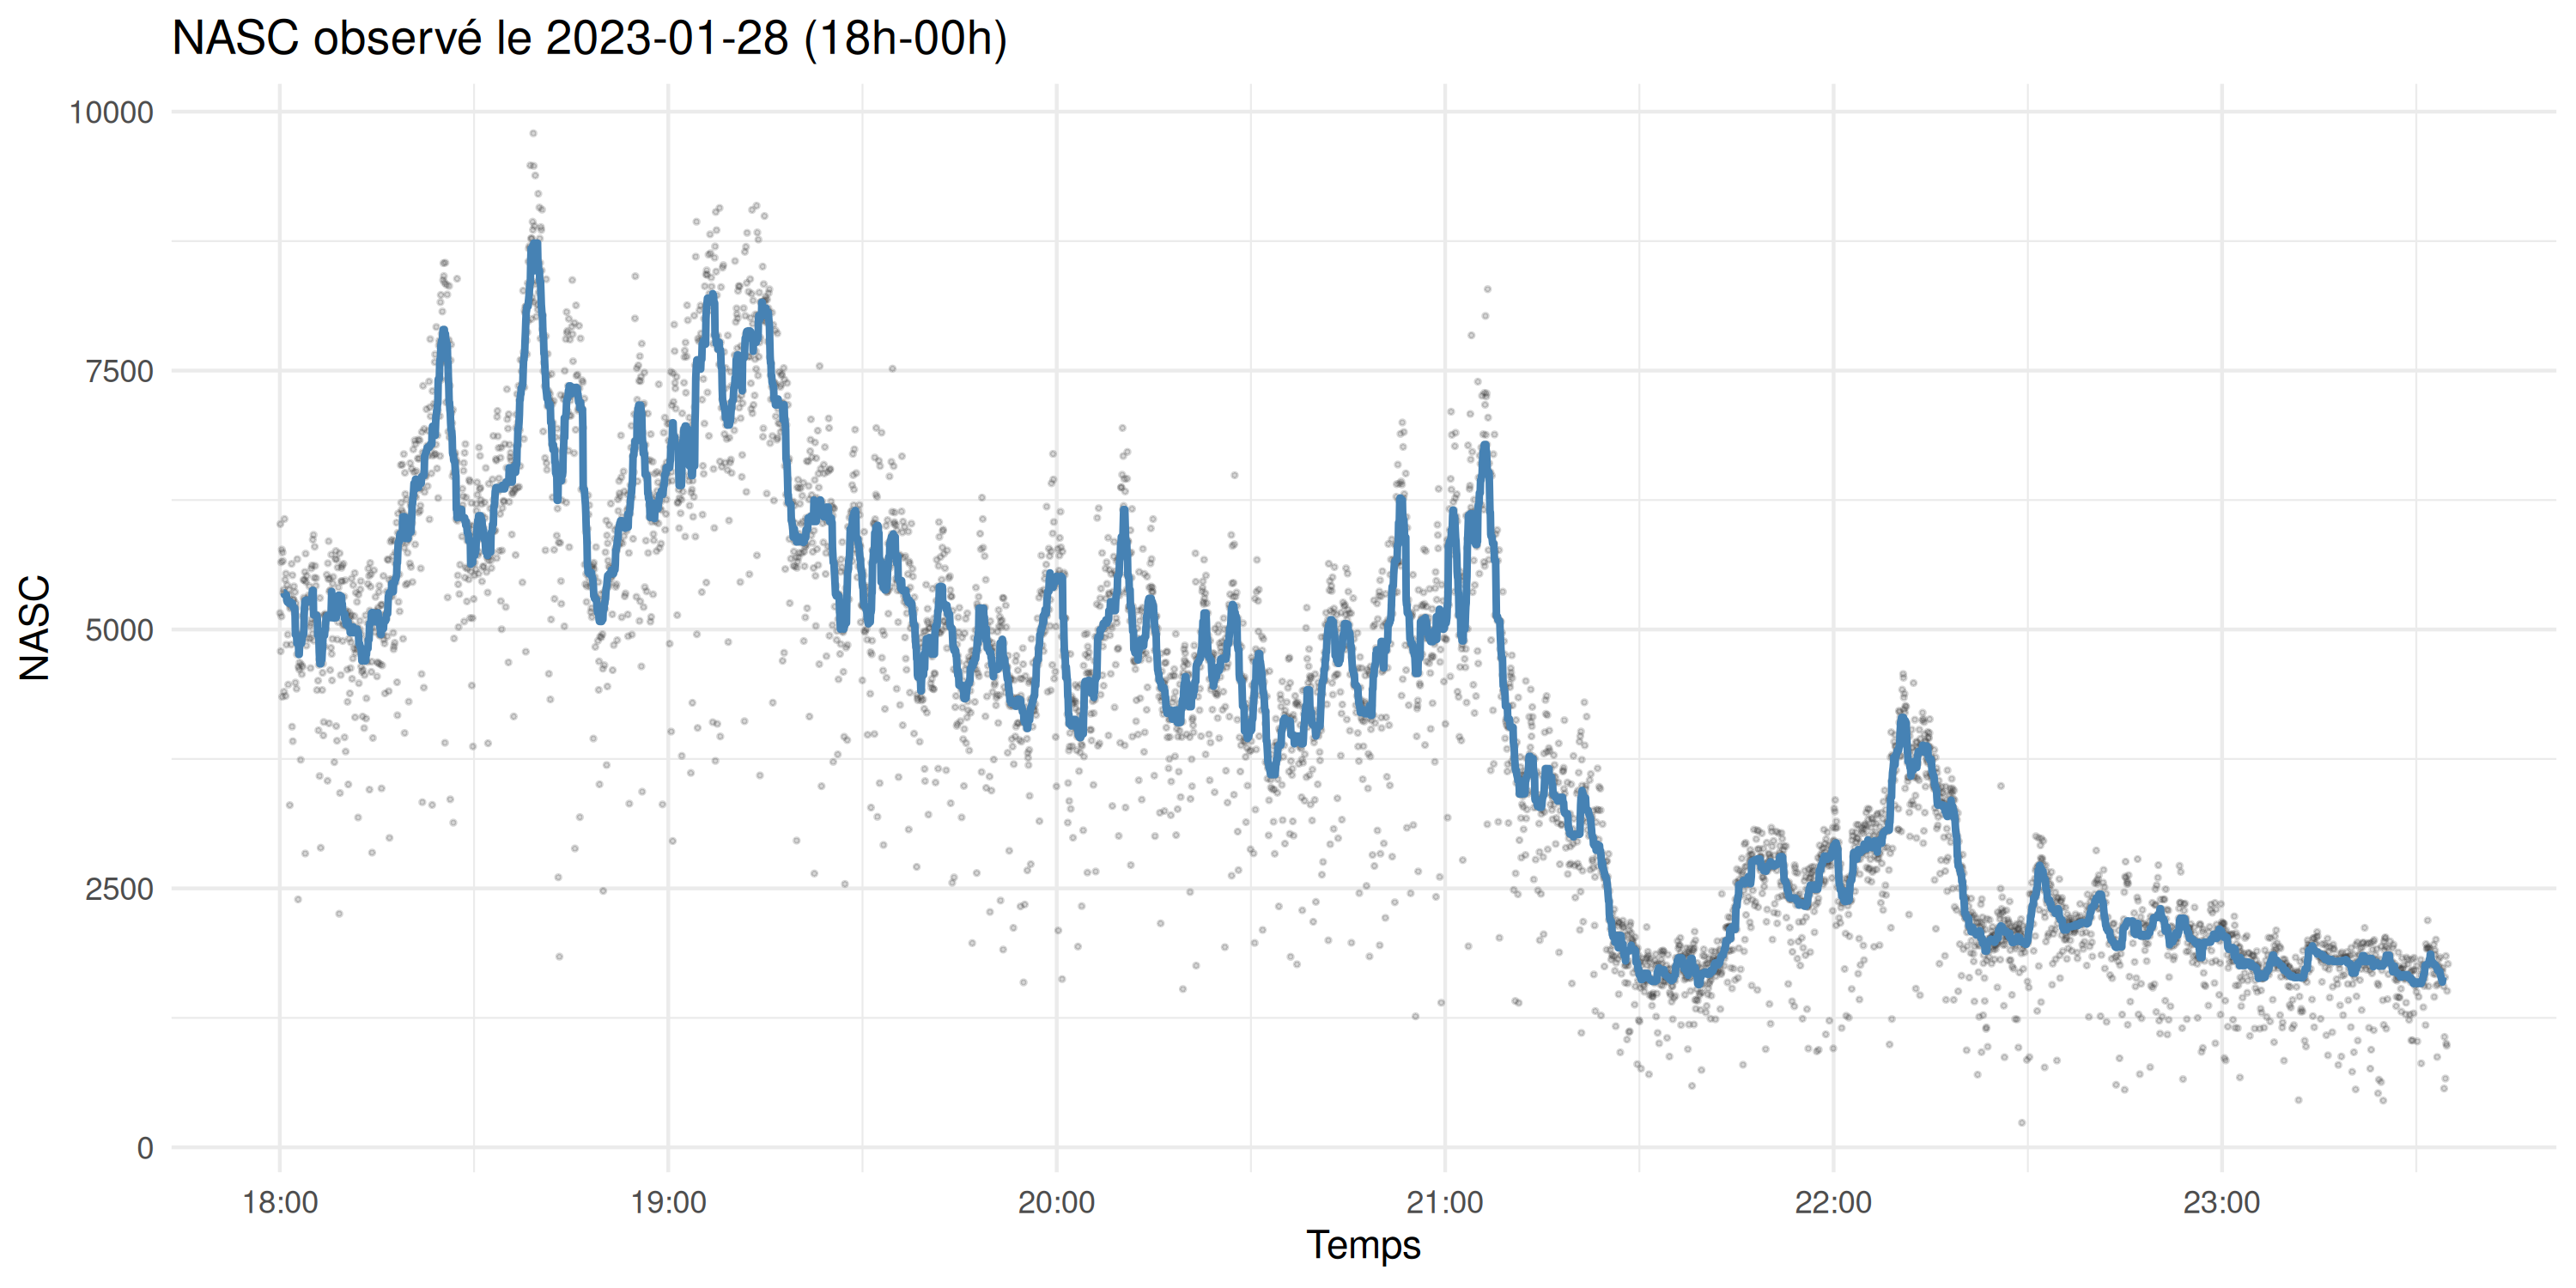
\includegraphics[width=0.7\textwidth]{images/02_materiel_et_methode/active_acoustic_et_NASC/nasc_2023-01-28_smooth_bis}
		\caption{NASC en fonction du temps le 2023-01-28, données d'acoustique active (transect) issues de la campagne océanographique OBSAUSTRAL 2023 \cite{flotteoceanographique_campagnes}.}
		\label{fig:nasc}
	\end{figure}
	 
 
 
 
 
 
 
 
 
 \section{Concentrations de pigments photosynthétiques (PIGMeANN)}
	 La couleur des océans dépend de leur composition en pigments et ces pigments sont contenus dans les organismes phytoplanctoniques. L'analyse de la couleur des océans à partir d'images satellite permet donc d'étudier les communautés phytoplanctoniques sur une échelle spatiale et temporelle large. L'algorithme PIGMeANN \cite{sari2026regional} associe, à l'aide de réseaux neuronaux profonds, une empreinte spectrale \footnote{Forme caractéristique du spectre de la lumière réfléchie par l'eau, c'est-à-dire de la façon dont la réflectance varie selon la longueur d'onde. Chaque pigment absorbe la lumière à des longueurs d'onde précises : des communautés de composition pigmentaire différente produisent donc des spectres de forme différente.} à des mesures de concentrations de pigments phytoplanctoniques \textit{in-situ} obtenues par High Performance Liquid Chromatography (HPLC) \footnote{Permet de séparer et quantifier les pigments afin d’identifier les différents groupes phytoplanctoniques présents. L’échantillon est injecté dans une colonne traversée par un solvant sous haute pression, où ses différents composés sont séparés puis détectés individuellement.}. Ainsi, cette méthode permet de prédire les concentrations de neuf pigments phytoplanctoniques sur l'ensemble de la ROI. Ils sont détaillés dans le tableau \ref{tab:pigments}.
	
	\begin{table}[H]
		\centering
		\footnotesize
		\setlength{\tabcolsep}{3pt}
		\renewcommand{\arraystretch}{1.3}
		\begin{tabularx}{\textwidth}{
				>{\raggedright\arraybackslash}p{1.3cm}
				*{9}{>{\centering\arraybackslash}X}
			}
			\hline
			\textbf{Pigment} & Divinyl chloro\-phylle $a$ & Chloro\-phylle $a$ & Chloro\-phylle $b$ & Zéaxan\-thine & Fucoxan\-thine & 19'-hexanoyl\-oxyfuco\-xanthine & 19'-butanoyl\-oxyfuco\-xanthine & Allo\-xanthine & Péri\-dinine \\
			\hline
		\end{tabularx}
		\renewcommand{\arraystretch}{1}
		\caption{Neuf pigments photosynthétiques dont les concentrations sont estimées par l'algorithme PIGMeANN \cite{sari2026regional}.}
		\label{tab:pigments}
	\end{table}
	
	La figure  \ref{fig:mapchla2023-01-26} illustre la prédiction par PIGMeANN de la Chorophylle-a le 2023-01-26 sur le secteur étudié. Les zones non colorées correspondent sont des données manquantes. La forte couverture nuageuse de la région induit une absence de données satellitaires, et donc des concentrations prédites par PIGMeANN.
	 
	\begin{figure}[H]
		\centering
		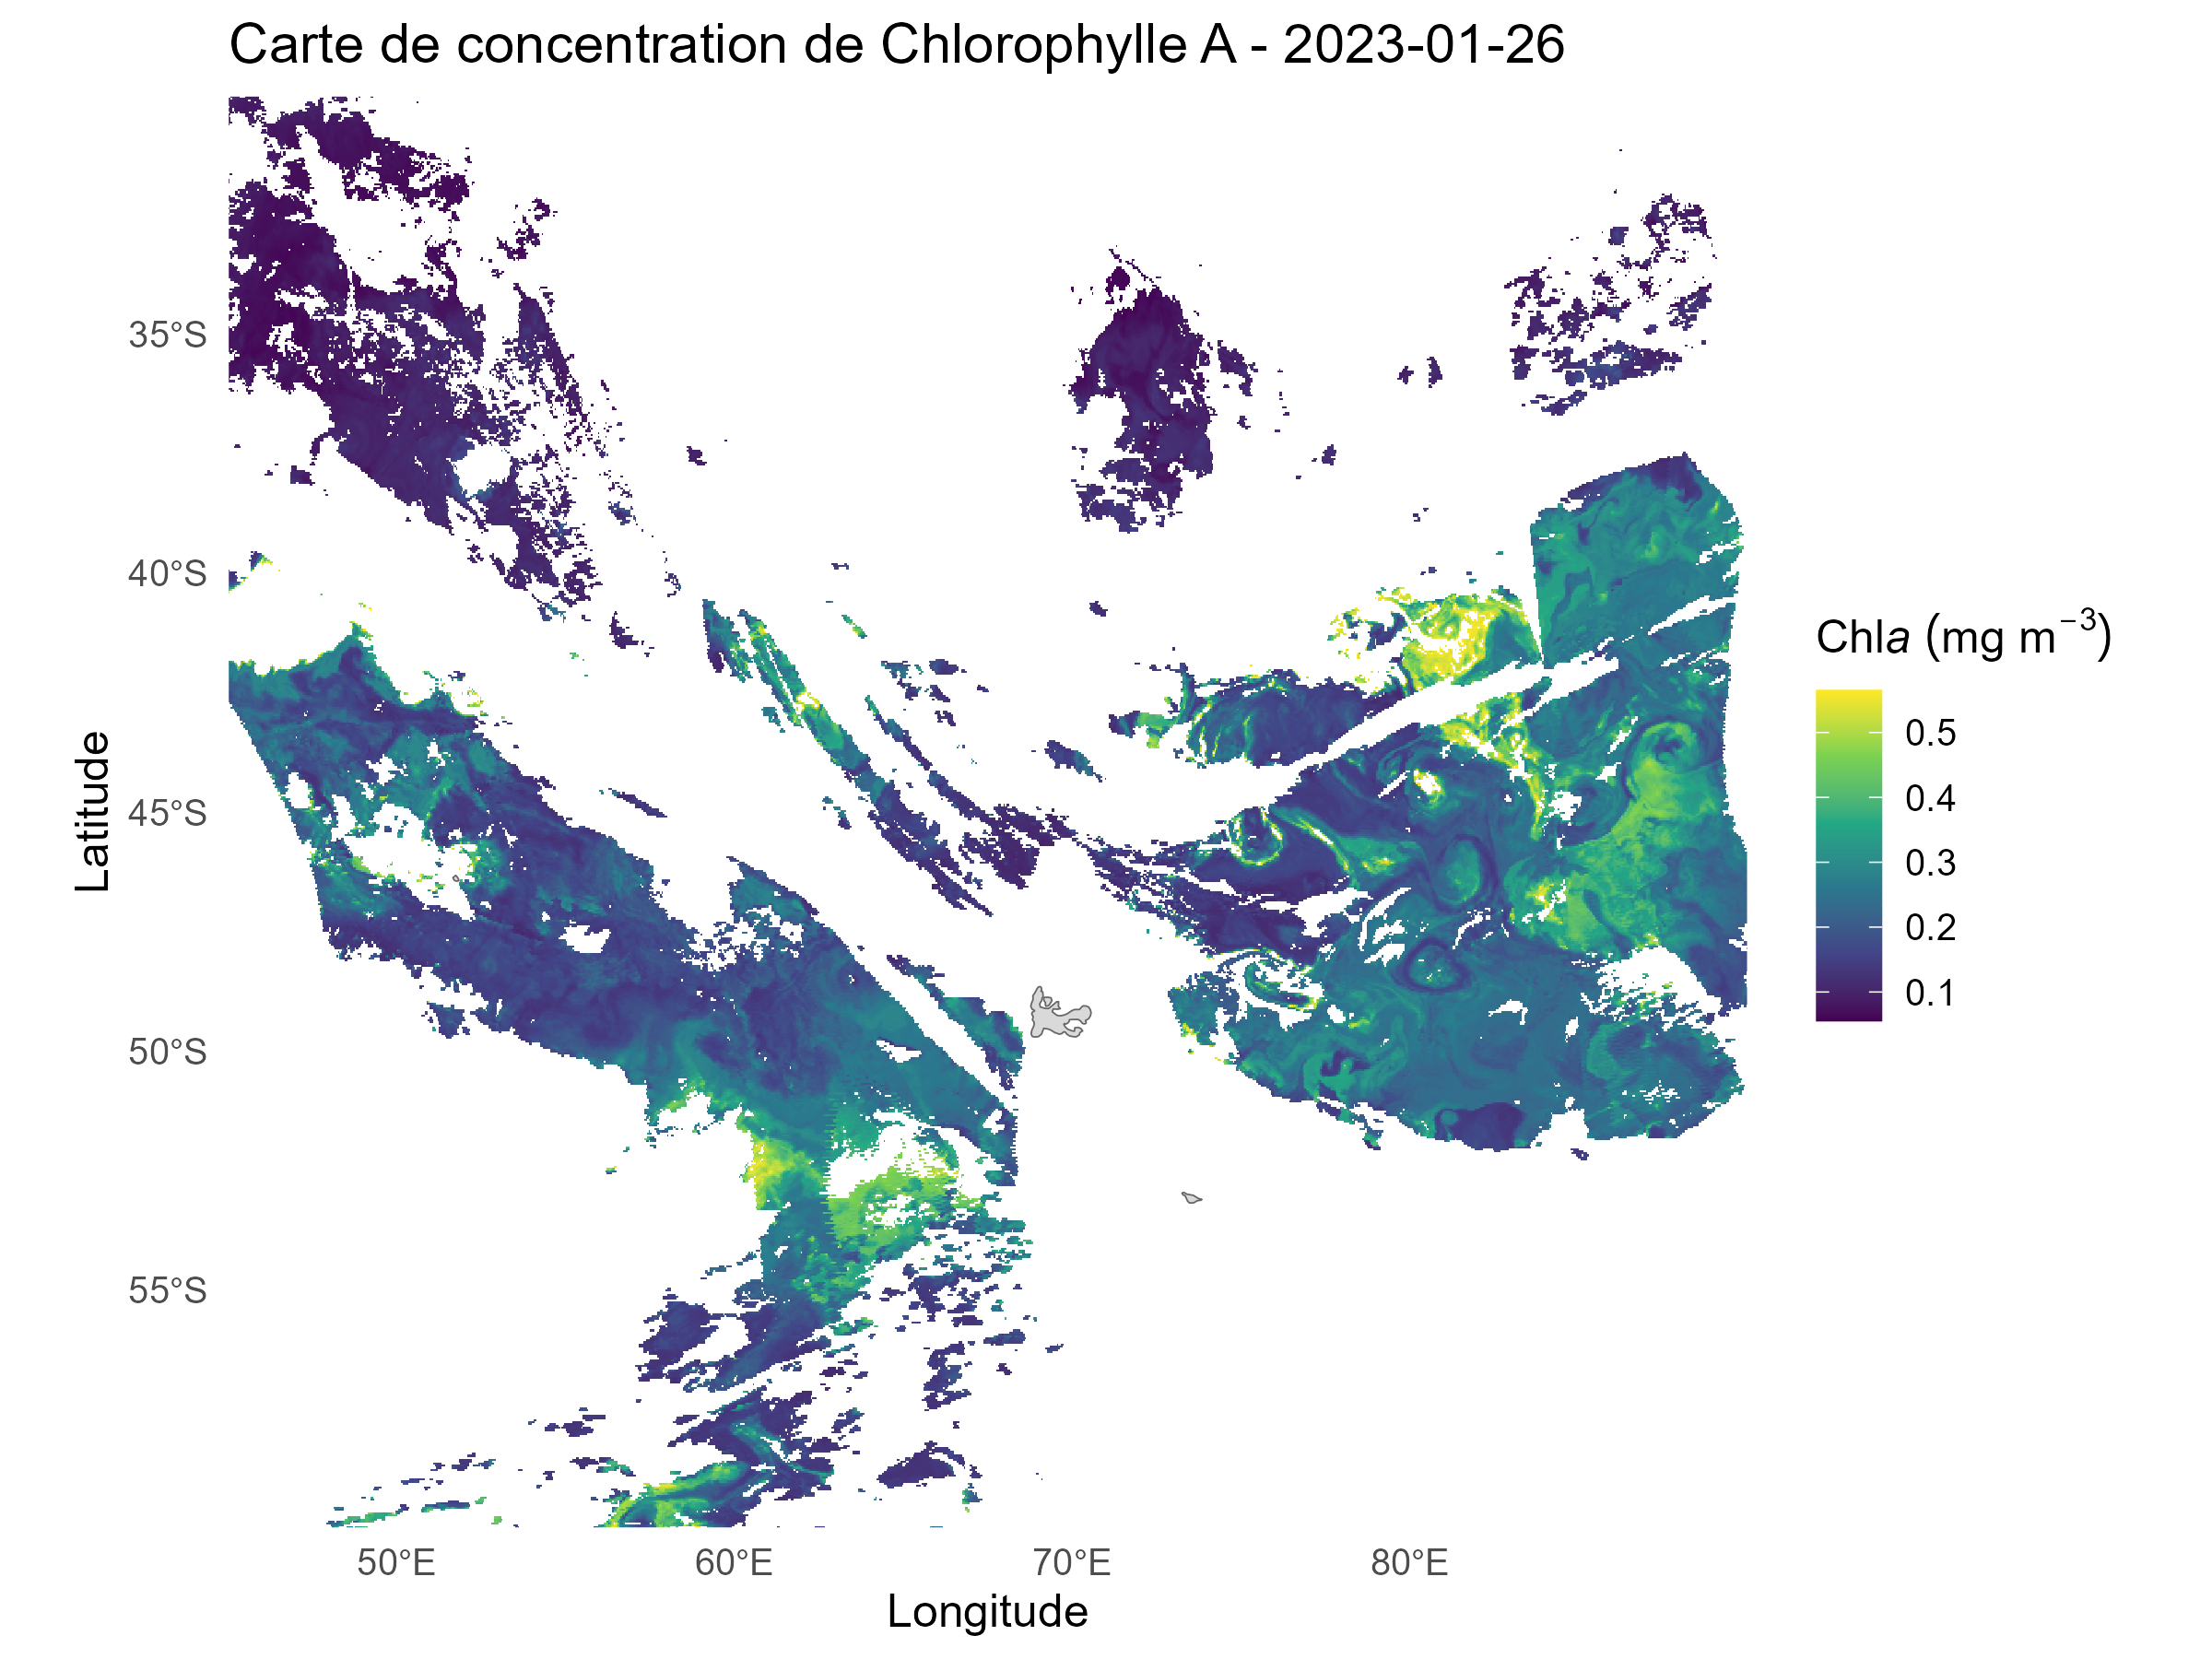
\includegraphics[width=0.7\textwidth]{images/02_materiel_et_methode/map_chla_2023-01-26}
		\caption{Carte de prédiction de la concentration de Chlorophylle-a le 2023-01-26 sur le secteur indient du SO, prédictions issue de l'alorithme PIGMeANN développé par Sari el Dine \cite{sari2026regional}. La présence de nuages gène grandement la prédiction sur la zone totale.}
		\label{fig:mapchla2023-01-26}
	\end{figure}
	 
	Plutôt que les concentrations pigmentaires absolues, on s'intéresse aux concentrations relative, c'est-à-dire le ratio des concentrations de pigments sur la somme des concentrations pigmentaires totale (Chlorophylle-a exclue \footnote{ubiquitaire, elle n'apporte pas d'information sur la composition de la communauté}) :
	 
	 \begin{equation}
	 	R_i = \frac{[\text{Pigment}_i]}{\displaystyle\sum_{j \neq \text{Chla}} [\text{Pigment}_j]}
	 	\label{eq:ratio_pigment}
	 \end{equation}
	 
	 La concentration relative $R_i$ la plus importante à une certaine localisation et temps permet d'identifier hypothétiquement les classes taxonomique (Phytoplanctonique Functional Types, PFT) ou de taille (Phytoplanctonic Size Class, PSC)  dominantes de la communauté, par association avec les connaissances théoriques développées dans la littérature \cite{sari2025influence}, \cite{heidemann2024drivers} \cite{Georges2014}. Ces correspondances sont détaillées dans le tableau \ref{tab:corresp_pig}. L'abondance totale de phytoplancton est estimée par la concentration absolue en Chlorophylle-a, pigment ubiquitaire présent chez la majorité des organismes photosynthétiques.
	 % J'hésite à mettre ça en Discussion
 
 	\begin{table}[H]
 		\centering
 		\renewcommand{\arraystretch}{1.3}
 		\begin{tabular}{
 				>{\raggedright\arraybackslash}p{3.4cm}
 				>{\raggedright\arraybackslash}p{2.0cm}
 				>{\raggedright\arraybackslash}p{4.8cm}
 				>{\raggedright\arraybackslash}p{2.6cm}
 			}
 			\hline
 			\textbf{Pigment} & \textbf{Abréviation} & \textbf{Groupe phytoplanctonique associé (PFD)} & \textbf{Classe de taille (PSC)} \\
 			\hline
 			Divinyl chlorophylle $a$ & dvChla & Procaryotes picoplanctoniques (\textit{Prochlorococcus}) & Picophytoplancton \\
 			Chlorophylle $a$ & Chla & Marqueur de biomasse totale (tous groupes) & -- \\
 			Chlorophylle $b$ & Chlb & Chlorophycées / Prasinophycées & Picophytoplancton \\
 			Zéaxanthine & Zea & Cyanobactéries (\textit{Synechococcus}) & Picophytoplancton \\
 			Fucoxanthine & Fuco & Diatomées (dominantes) & Microphytoplancton \\
 			19'-hexanoyloxyfucoxanthine & Hex & Prymnésiophycées (haptophytes) & Nanophytoplancton \\
 			19'-butanoyloxyfucoxanthine & But & Prymnésiophycées / pélagophytes & Nanophytoplancton \\
 			Alloxanthine & Allo & Cryptophycées & Nanophytoplancton \\
 			Péridinine & Per & Dinoflagellés (péridiniens) & Microphytoplancton \\
 			\hline
 		\end{tabular}
 		\renewcommand{\arraystretch}{1}
 		\caption{Pigments photosynthétiques analysés et groupes phytoplanctoniques hypothétiquement associés (PFD et PSC) dans le secteur de Kerguelen en été austral, d'après \cite{Lasbleiz2014}, \cite{sari2025influence}}
 		\label{tab:corresp_pig}
 	\end{table}
 
 \section{Données modèles de température et salinité (CMEMS) et calcul des Domaines Océanographiques Fonctionnels (FOD)}
	 \subsection{Données modèles de température et salinité (CMEMS)}
		\label{section:temp_sal}
		 Les données de températures et salinité font partie du jeu de données "Global Ocean Physics Reanalysis" (la réanalyse GLORYS12V1, GLOBAL\_MULTIYEAR\_PHY\_001\_030) \cite{cmems_glorys12}, issues de la plateforme Copernicus \footnote{Programme d’observation de la Terre de l’Union européenne, qui fournit notamment des données et services permettant de surveiller et comprendre l’état de l’environnement, dont l’océan \cite{copernicus2026services}}. Ce sont des données issues des observations temps-réelles CMEMS \footnote{Copernicus Marine Environment Monitoring Service, service marin de Copernicus} et réanalysées par le modèle NEMO \footnote{Nucleus for European Modelling of the Ocean, modèle numérique de l’océan qui simule l’évolution de paramètres comme la température, la salinité, les courants et le niveau de la mer}, et ERA5 \footnote{Modèle atmosphérique de l'ECMWF (European Centre for Medium-Range Weather Forecasts) qui fournit les conditions atmosphériques nécessaires pour forcer le modèle océanique NEMO à sa surface}. Elles ont une résolution spatiale de 0.083° et une résolution temporelle journalière.
		 Afin d'alléger le traitement des données, seules les mesures de température et de salinité comprises entre 20 et 500 m de profondeur ont été conservées. La figure \ref{fig:T_S_profile} présente un exemple de profile de température et salinité à 50°E de longitude, 60°S de latitude, le 2023-01-26.
		\begin{figure}[H]
			\centering
			\includegraphics[width=\linewidth]{images/02\_materiel\_et\_methode/TS\_FOD/profils\_TS\_2023-01-26.png}
			\caption{Profil de Température et de Salinité issue de GLORYS (CMEMS), tronqués en deçà de 20m et au delà de 500m aux coordonnés (50°E, 60°S).}
			\label{fig:T_S_profile}
		\end{figure}
 
 	\subsection{Calcul des Domaines Océanographiques Fonctionnels (FOD)}
	 	Les Domaines Océanographiques Fonctionels (FOD, Functional Oceanographic Domain) sont des masses d'eau ayant des caractéristiques thermohalines similaires. La méthode d'identification des FOD a été développée par Fonvieille N. et Nerini D. \cite{fonvieille2024}. Les profils de température et salinité sont, dans un premier temps (1), estimées dans un espace fonctionnel par projection sur une base de B-spline. Dans un second temps (2), la dimension de la matrice des coefficients de pondération des B-splines est réduite par Analyse par Composante Principale (PCA, Principal Componant Analysis). Dans un dernier temps (3), un clustering (GMM) est appliqué à $K$ composantes principales déterminé par la PCA de l'étape précédente. Ces trois étapes sont développées en Annexe \ref{annexe:methode_fod}.
	 	
	 	\vspace{0.3cm}
	 	
	 	Dans notre étude, l'estimation par projection sur une base de B-splines a été effectué avec l'hyperparamètre de régularisation $\lambda = 0.25$, pour $K=25$ B-splines. Sont conservées pour le clustering 6 composantes principales ($>0.99$ \% explained var., voir tableau \ref{tab:pca_variance}). L'indice BIC nous permet de sélectionner $nclust = 6$ clusters. En ajoutant les classes de transitions (les soft classes, c'est-à-dire toutes les données dont la probabilité d'appartenance au cluster le plus probable est inférieure à $thr  = 0.75$), on obtient alors 13 clusters distincts (7 clusters de "transitions") \footnote{La classe "NA" correspond aux clusters manquants sur le plateau de Kerguelen. Les profils de température et salinité allant de 20 à 500m, sont retirés des calculs tout profils ayant des données manquantes entre ces deux valeurs. Les zones où la bathymétrie est inférieure à 500m sont donc exclues de ces calculs.}, ce sont les 13 Domaines Océanographiques Fonctionnels (FOD).
	 	
		\begin{figure}[H]
			\centering
			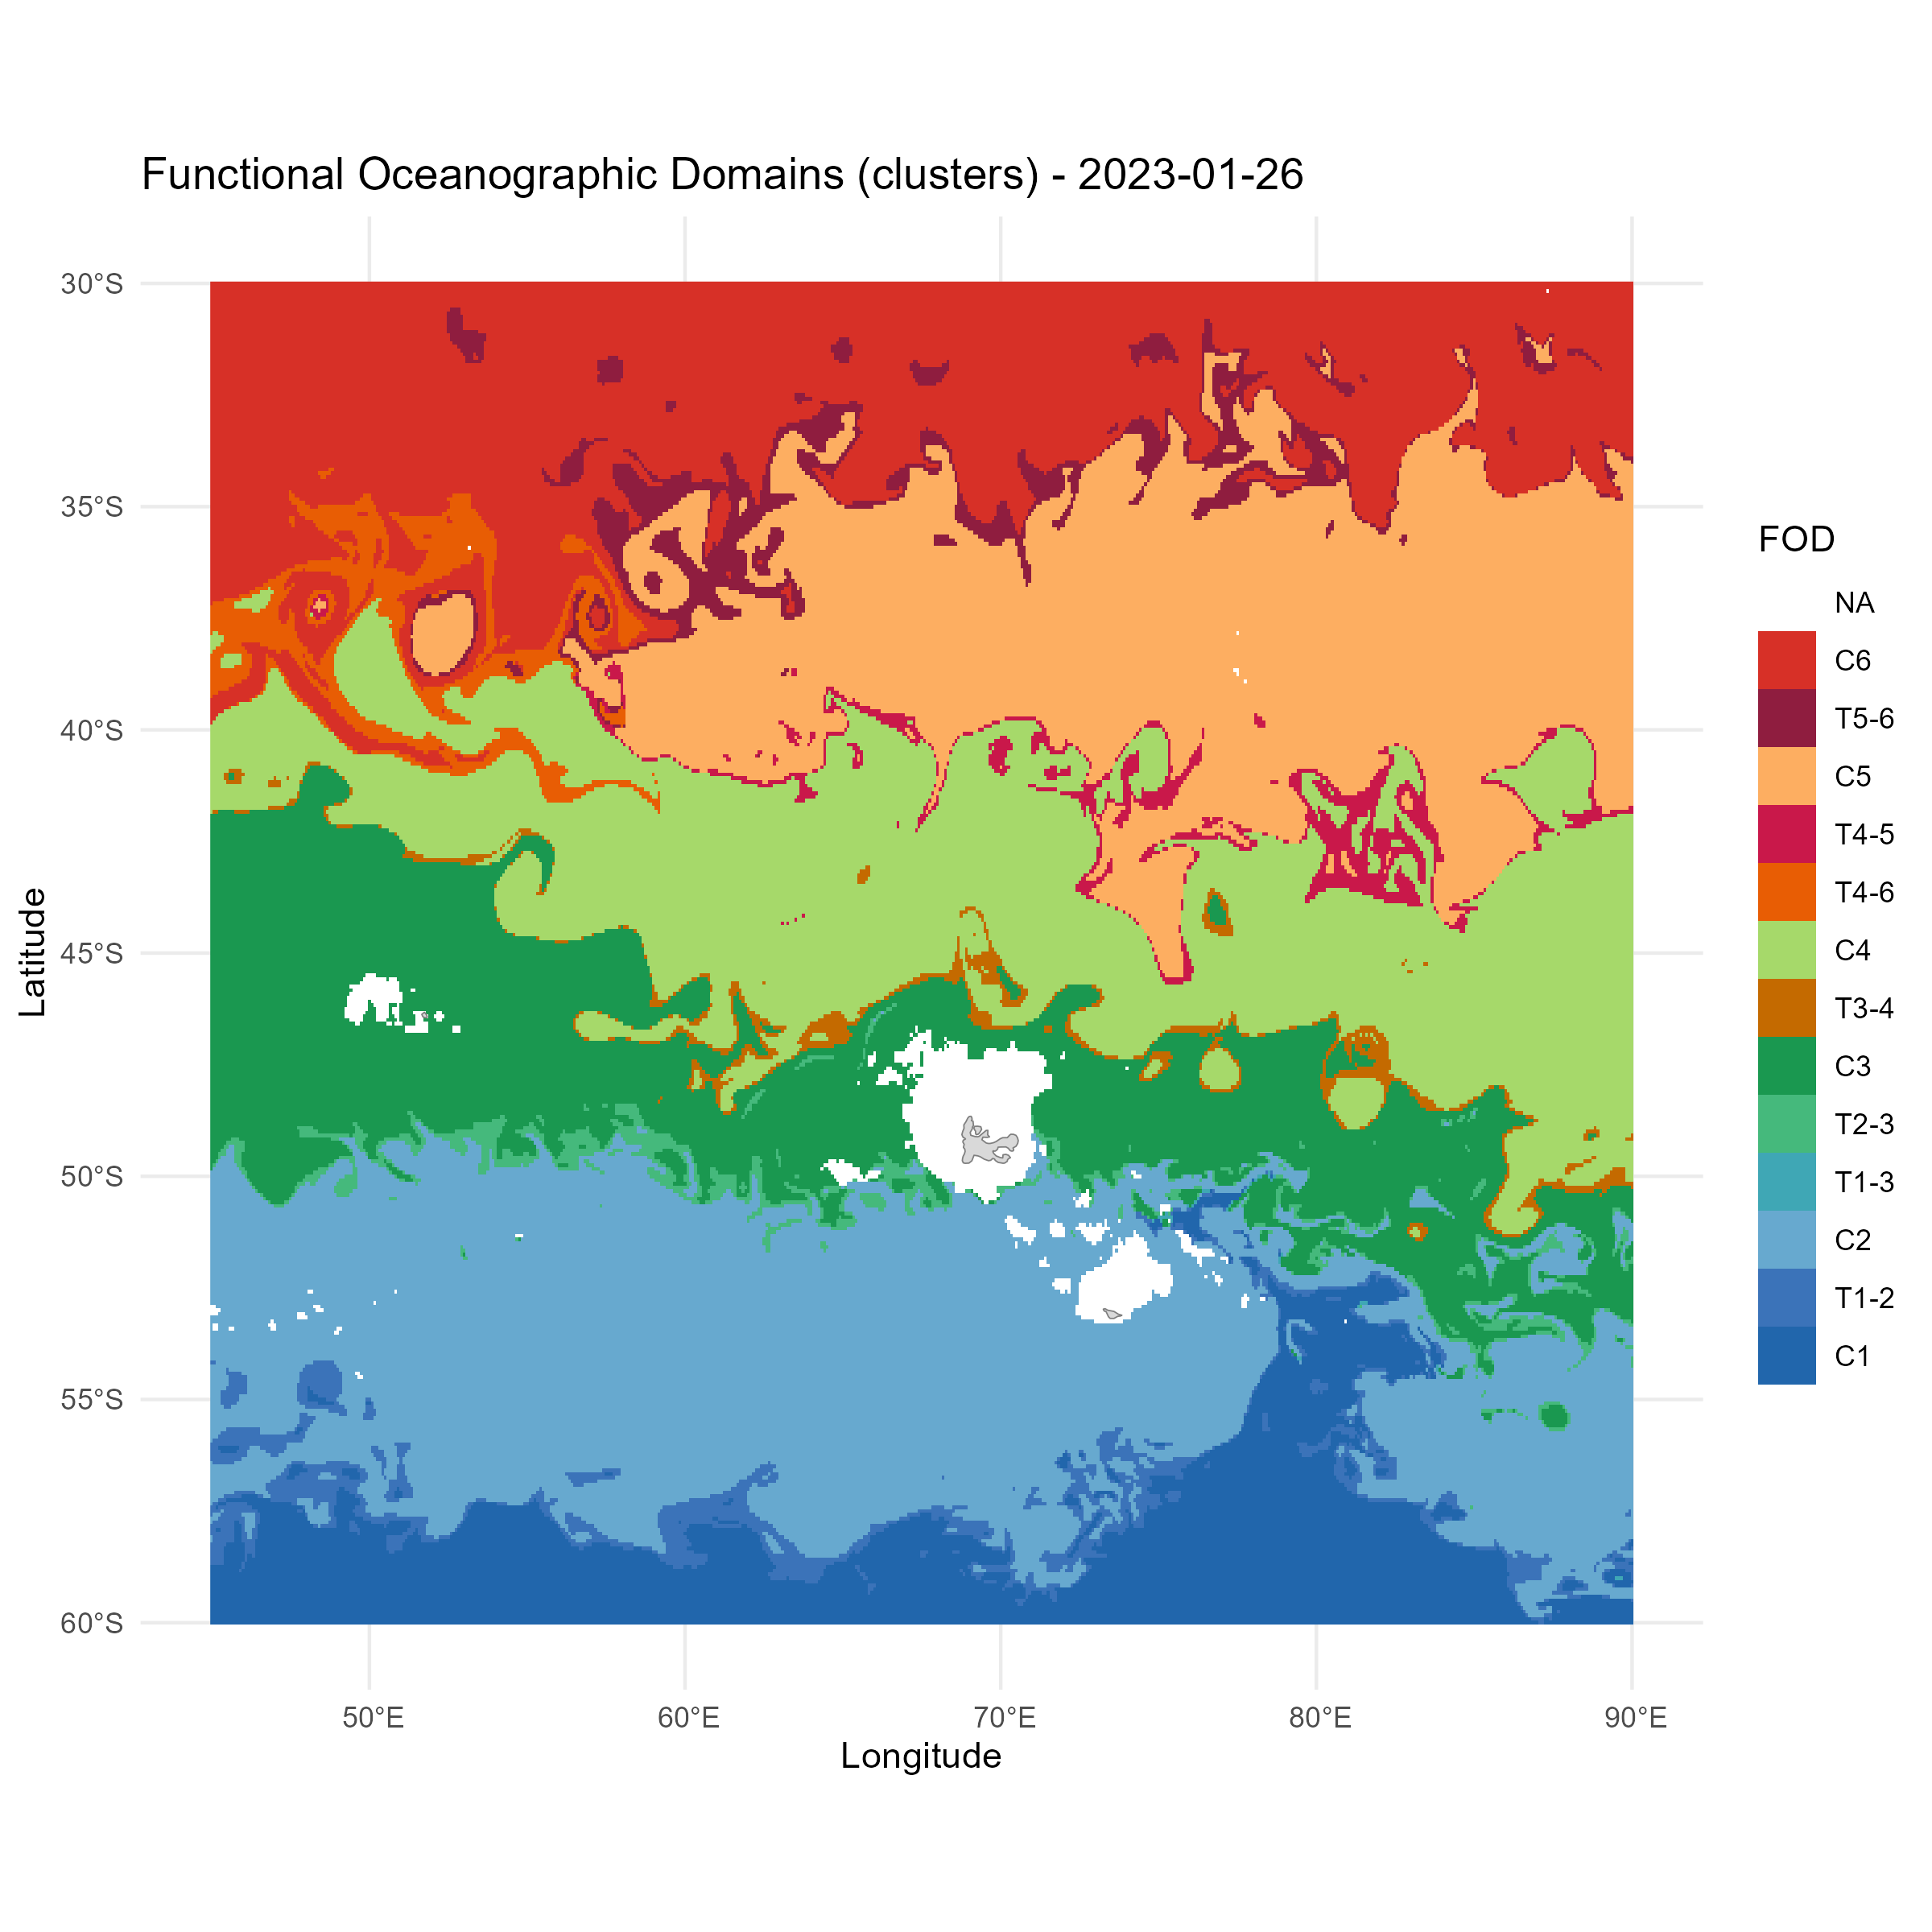
\includegraphics[width=0.8\textwidth]{images/02_materiel_et_methode/TS_FOD/cluster_transition_map_renamed_20230126}
			\caption{Carte des Domaines Océanographiques Fonctionnels du 2023-01-26 générée par la méthode développée par Fonvieille N. et Nerini D. \cite{fonvieille2024}.}
			\label{fig:fodmap}
		\end{figure}
		
	 	\begin{figure}[H]
	 		\centering
	 		\begin{subfigure}[b]{0.48\textwidth}
	 			\centering
	 			\includegraphics[width=0.7\textwidth]{images/02\_materiel\_et\_methode/TS\_FOD/temperature\_clusters\_transitions.png}
	 			\caption{Profil de température (°C) moyen par cluster}
	 		\end{subfigure}
	 		\hfill
	 		\begin{subfigure}[b]{0.48\textwidth}
	 			\centering
	 			\includegraphics[width=0.7\textwidth]{images/02\_materiel\_et\_methode/TS\_FOD/salinity\_clusters\_transitions.png}
	 			\caption{Profil de salinité (PSU) moyen par cluster}
	 		\end{subfigure}
	 		\caption{}
	 		\label{fig:temp_sal_cluster}
	 	\end{figure}
	 	
	 	 La figure \ref{fig:fodmap} illustre les 13 FOD capturés le 2023-01-26. Pour chacun des FOD, les profils de température et de salinité moyennés sur l'ensemble de la période d'étude sont présentés en figure \ref{temp_sal_cluster}. Chaque FOD correspond donc une masse d'eau ayant des propriétés thermohalines similaires. La projection de ces FOD sur une carte permet également de visualiser l'hydrodynamisme de la région. Les fronts sont des zones de rencontres entre des masses d'eau ayant propriétés hydologiques différentes. Les FOD de "transition" permettent de les identifier : T2-3 correspond à la transition entre le cluster 2 et le cluster 3. Sa latitude ($\approx 50$°S) permet de l'identifier comme Front Polaire. En suivant la même méthode, on peut identifier le Front Subantarctique (T3-4) et le front sub-tropical (T4-5/T4-6). Les tourbillons sont des courants en vortex, ce qui empêche les masses d'eau de se mélanger entre elles. Ainsi, on peut également identifier les tourbillons sur les cartes de FOD : ce sont les régions où, localement, un FOD est présent, entouré par un autre FOD dominant. Sur la figure \ref{fig:fodmap}, on remarque par exemple un tourbillon aux coordonnées (53°E, 27°S) environ : le cluster 5 est pris dans un tourbillon.
 	
 \section{Champs de courants modèles (CMEMS) et calcul du Finite Time Lyapunov Exponent (FTLE)}
 \subsection{Données de Champs de courants modèles (CMEMS)}
 	Les champs de courants sont des données modèles également issues du modèle de réanalyse océanique GLORYS12 du Copernicus Marine Service (CMEMS), détaillé en section \ref{section:temp_sal}. Les champs de courants de surface (composantes zonale (u) et méridienne (v)) en sont extraits avec une résolution journalière.  
 	
 \subsection{Calcul du Finite-Time Lyapunov Exponent}
	 Le Finite Time Lyapunov Exponent est un indicateur qui permet de caractériser la séparation ou la convergence de trajectoires de particules d’eau sur une durée finie. On peut ainsi identifier les structures dynamiques susceptibles de contrôler le transport et la dispersion dans l’océan \cite{shadden2005definition}, \cite{dovidio2004mixing}. Son calcul, effectué dans cette étude par Molinet M. \footnote{Doctorant au MIO et CEBC, encadrant de ce stage} est le suivant :
	 
	 On considère le champ de vitesse bidimensionnel dépendant de la position et du temps, issu des données de réanalyse GLORYS21 :
	 \begin{equation}
	 	\mathbf{u}(x,y,t)
	 	=
	 	\begin{pmatrix}
	 		u(x,y,t)\\
	 		v(x,y,t)
	 	\end{pmatrix}
	 \end{equation}
	 avec $u$ et $v$ représentant respectivement les composantes zonale et méridienne de la vitesse, et où $\mathbf{x}=(x,y)$ désigne la position de la particule.
	 
	 À partir d'une position initiale $\mathbf{x}_0$ au temps $t_0$, la trajectoire d'une particule est obtenue en intégrant, dans notre cas avec la méthode Runge-kutta (RK4), l'équation d'advection :
	 
	 \begin{equation}
	 	\frac{d\mathbf{x}}{dt}
	 	=
	 	\mathbf{u}(\mathbf{x},t),
	 	\qquad
	 	\mathbf{x}(t_0)=\mathbf{x}_0.
	 \end{equation}
	 
	 Après une durée d'intégration $T$, la position finale de la particule peut être décrite à l'aide du flot lagrangien :
	 
	 \begin{equation}
	 	\mathbf{x}(t_0+T)
	 	=
	 	\mathbf{F}_{t_0}^{T}(\mathbf{x}_0),
	 \end{equation}
	 
	 où $\mathbf{F}_{t_0}^{T}$ est l'application qui associe à chaque position initiale $\mathbf{x}_0$ sa position après une durée $T$.
	 
	 On peut ensuite analyser la variation des trajectoires $\mathbf{F}_{t_0}^T(x_0)$ après un temps $T$ si l'on change la position initiale $x_0$ des particules (tenseur de déformation): 
	 \begin{equation}
	 	\nabla \mathbf{F}_{t_0}^{T}
	 	=
	 	\frac{\partial \mathbf{F}_{t_0}^{T}}{\partial \mathbf{x}_0}
	 	=
	 	\begin{pmatrix}
	 		\frac{\partial F_x}{\partial x_0} &
	 		\frac{\partial F_x}{\partial y_0} \\[6pt]
	 		\frac{\partial F_y}{\partial x_0} &
	 		\frac{\partial F_y}{\partial y_0}
	 	\end{pmatrix}
	 \end{equation}
	 
	 Le tenseur de Cauchy-Green permet de quantifier la déformation des distances entre des particules initialement proches. Il est défini par :
	 \begin{equation}
	 	\mathbf{C}_{t_0}^{T}(\mathbf{x}0)
	 	=
	 	\left(
	 	\nabla\mathbf{F}{t_0}^{T}(\mathbf{x}0)
	 	\right)^{T}
	 	\nabla\mathbf{F}{t_0}^{T}(\mathbf{x}_0).
	 \end{equation}
	 
	 Le facteur maximal d'étirement entre les particules est donné par la plus grande valeur popre $\lambda_{max}$ du tenseur de Cauchy-Green $\mathbf{C}_{t_0}^{T} (\mathbf{x}_0)$
	 
	 Le FTLE ($\sigma_{t_0}^{T}$) est ensuite calculé, il correspond au taux de croissance logarithmique du facteur d'étirement maximal $\lambda_{max}$, normalisé par la durée d'intégration $T$ :
	 
	 \begin{equation}
	 	\sigma_{t_0}^{T}(\mathbf{x}_0)
	 	=
	 	\frac{1}{|T|}
	 	\ln\left(
	 	\sqrt{
	 		\lambda_{\max}\left(
	 		\mathbf{C}_{t_0}^{T}(\mathbf{x}_0)
	 		\right)
	 	}
	 	\right)
	 \end{equation}
	 
	 avec :
	 \begin{itemize}
	 	\item $\mathbf{C}_{t_0}^{T}$ le tenseur de Cauchy-Green, décrit comment les distances entre les particules évoluent. Il est calculé à partir des données de champs de courants
	 	\begin{equation}
	 		\mathbf{C}_{t_0}^{T}
	 		=
	 		\left(\nabla\mathbf{F}_{t_0}^{T}\right)^{T}
	 		\left(\nabla\mathbf{F}_{t_0}^{T}\right)
	 	\end{equation}
	 	\item $	\lambda_{\max}$ la plus grande valeur propre du tenseur de Cauchy-Green
	 	\item $\mathbf{x}_0$ la position initiale de la particule
	 	\item $T$ le tempsd d'intégration pendant lequel on suit la particule
	 	\item $\sigma$ le FTLE qui mesure le taux moyen de séparation des trajectoires des particules, exprimé en unité inverse du temps
	 \end{itemize}
	 
	 \vspace{0.5em}
	 
	\begin{figure}[H]
		\centering
		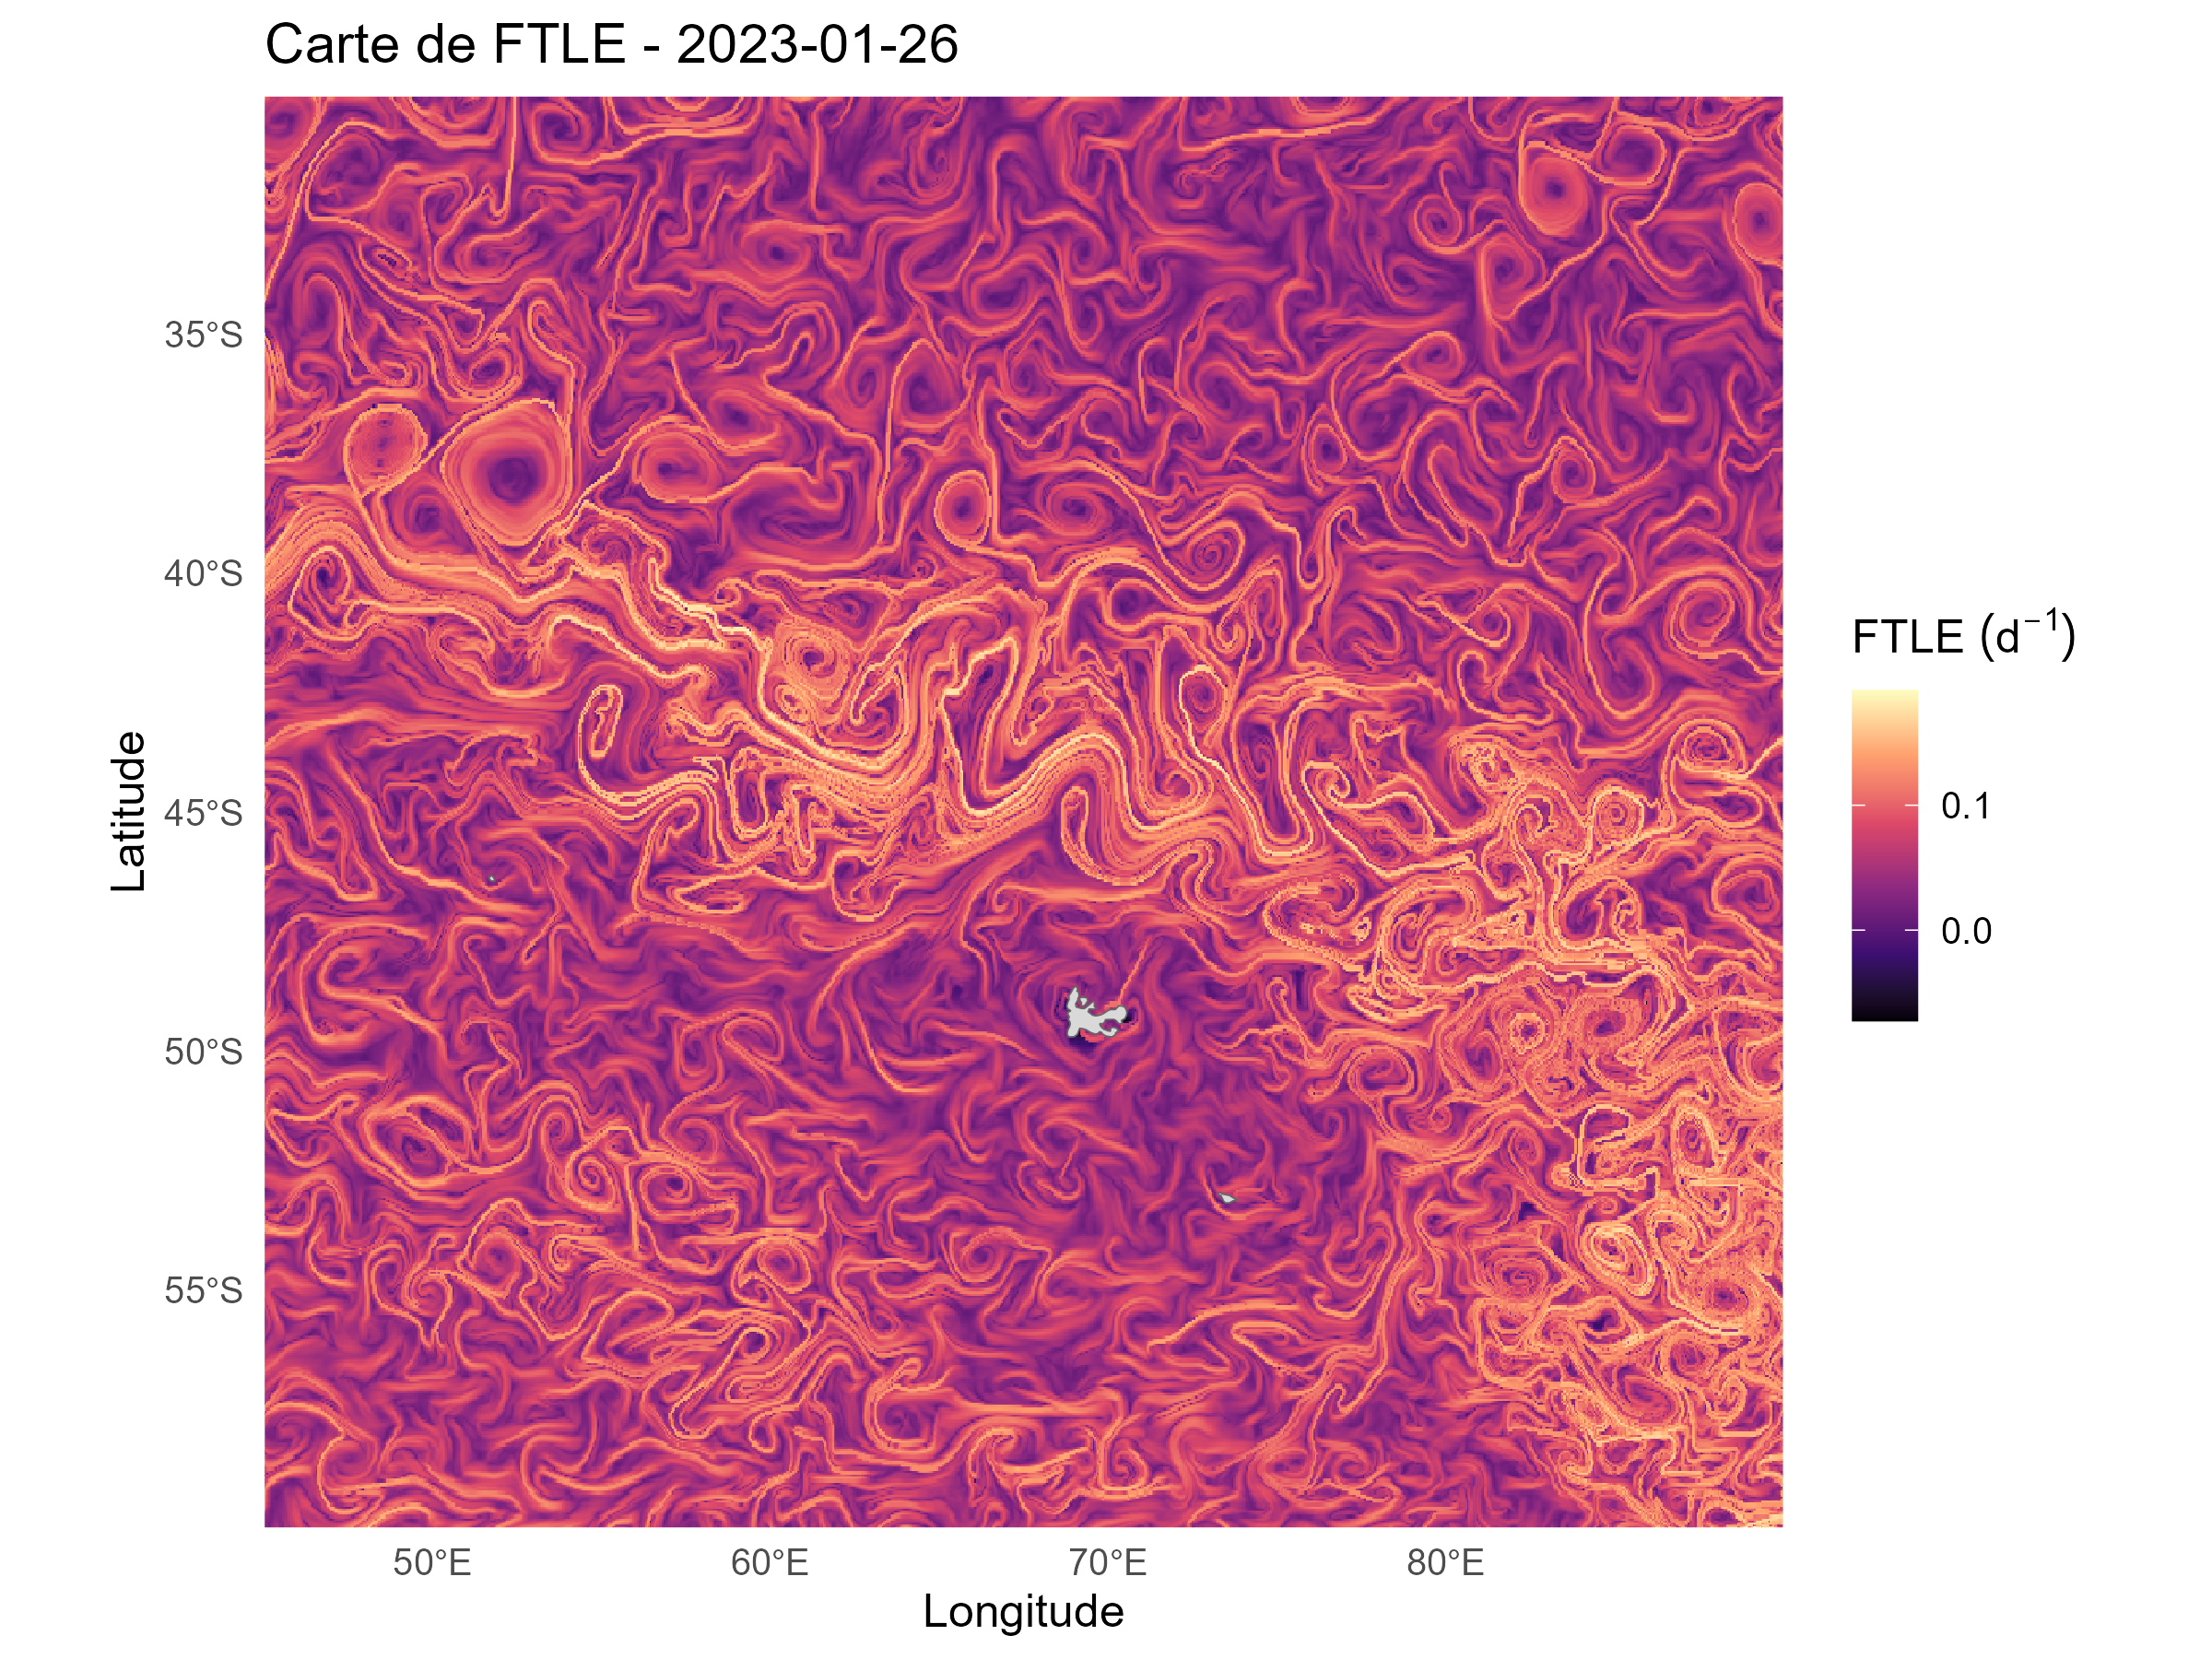
\includegraphics[width=0.5\textwidth]{images/02_materiel_et_methode/map_ftle_2023-01-26}
		\caption{Advection Lagrangienne FTLE backward (30j) du 2023-01-26. Les valeurs élevées de FTLE délimitent des crêtes correspondant à des frontières de transport de l'écoulement (de fronts ou de tourbillons) le long desquelles convergent les masses d'eau (structures cohérentes lagrangiennes attractives)}
		\label{fig:mapftle2023-01-26}
	\end{figure}
	 
	 Dans notre étude, la durée d'advection est de trente jours en backward, c'est-à-dire que les trajectoires sont intégrées vers l'arrière dans le temps (de $t$ à $t - T$). La résolution temporelle est journalière et la résolution spatiale est de 0.05°. La figure \ref{fig:mapftle2023-01-26} présente une carte de FTLE issue de la journée 2023-01-26. Les crêtes (valeur élevées) de FTLE marquent les zones où les particules voisines se séparent le plus fortement, ce qui permet d'identifier des structures physiques réelles de l'écoulement océanique.
	 
	 \subsection{Colocalisation des données par les plus proches voisins}
	\clearpage
	\chapter{Méthode}
Ce chapitre décris le protocole de validation des données et de modélisation du NASC par Forêts Aléatoires en fonction du FOD, FTLE et des ratios de concentrations pigmentaires : $NASC \sim FOD + FTLE + R_1, \ldots, R_9$. On décrira dans un premier temps le protocole de validation des données, puis, dans un second temps, le protocole d'apprentissage par Forêt Aléatoire (méthode, validation croisée, ajustement des hyperparamètres) suivi par l’évaluation du modèle, sa validation et enfin son interprétation.
	\section{Validation des données} % Analyse exploratoire des données (Exploratory Data Analysis, EDA)
	Les variables $NASC$, $FTLE$, $FOD$ et $R_1, \ldots, R_9$ sont des séries spatio-temporelles, acquises le long des trajets des campagnes océanographiques. Plusieurs de leurs propriétés peuvent compromettre l'apprentissage ou fausser l'évaluation du modèle : un échantillonnage déséquilibré ou informatif, des différences de distribution entre sous-ensembles de données, et une dépendance entre observations voisines. Cette section vise à caractériser ces propriétés indépendamment de tout modèle, afin (1) de justifier les choix de prétraitement, (2) de construire un schéma de validation croisée adapté et (3) de délimiter le domaine dans lequel les estimations du modèle pourront être interprétées.
	
	\paragraph{Notations}
		Les données sont constituées de $n$ unités élémentaires d'échantillonnage (\textit{Elementary Sampling Units}, ESU). Pour chaque ESU $i \in \{1, \dots, n\}$, on note :
		\begin{itemize}
			\item $Y_i \in \mathbb{R}_+$ la valeur du $NASC$ (variable cible) ;
			\item $X_i = (X_i^{(1)}, \dots, X_i^{(d)}) \in \mathbb{R}^d$ le vecteur des covariables ($FOD$, $FTLE$ et $R_1, \dots, R_9$, soit $d = 11$) ;
			\item $s_i \in \mathbb{R}^2$ la position de l'ESU, exprimée en degré de latitude et longitude ;
			\item $\tau_i \in \mathbb{R}$ l'instant d'acquisition ;
			\item $c_i \in \mathcal{C}$ la campagne océanographique d'acquisition.
		\end{itemize}
		Une partition naturelle des données est une partition $\{G_1, \dots, G_K\}$ de l'ensemble des indices $\{1, \dots, n\}$, dont chaque élément $G_k$ est appelé modalité. On considérera deux types de partitions : spatiale, où $G_k = \{i : s_i \in C_k\}$ pour une cellule $C_k$ d'une grille régulière couvrant la zone d'étude, et temporelle, où $G_k = \{i : c_i = c\}$ pour une campagne $c \in \mathcal{C}$. On note $n_k = |G_k|$ l'effectif de la modalité $k$.
	
	\subsection{Biais d'échantillonnage}
		Un biais d'échantillonnage peut affecter l'apprentissage de plusieurs manières. Par exemple : (1) une densité d'échantillonnage déséquilibrée conduit à un sous-apprentissage des conditions peu échantillonnées, et donc à une dégradation des performances prédictives dans ces conditions ; (2) lorsque la présence d'une observation dépend d'autres variables, voire de la valeur de la cible elle-même, les données disponibles ne sont plus représentatives de la population totale, ce qui induit un biais de sélection. Il est donc nécessaire d'identifier ces biais afin d'interpréter correctement les estimations du modèle et d'en encadrer la portée.
		
		Formellement, soit $S \in \{0, 1\}$ l'indicatrice d'échantillonnage d'un point $(s, \tau)$ du domaine d'étude. Les données observées sont issues de la loi conditionnelle $P(X, Y \mid S = 1)$, et non de la loi $P(X, Y)$ de la population. L'échantillonnage est dit \textit{ignorable} pour l'estimation de $f(x) = \mathbb{E}[Y \mid X = x]$ si $S$ est indépendant de $Y$ conditionnellement à $X$ :
		\begin{equation}\label{eq:ignorable}
			P(S = 1 \mid X, Y) = P(S = 1 \mid X).
		\end{equation}
		Dans ce cas, $\mathbb{E}[Y \mid X, S = 1] = \mathbb{E}[Y \mid X]$ et la relation apprise reste valable dans la population, même si la loi des covariables $P(X \mid S = 1)$ diffère de $P(X)$. Si au contraire la probabilité d'échantillonnage dépend de $Y$ (échantillonnage \textit{informatif}), l'estimateur appris est biaisé.
		
		Les données de $NASC$ sont des données \textit{in situ}, acquises lors des campagnes océanographiques OBSAUSTRAL/THEMISTO. % À compléter : origine des covariables (FTLE, FOD, ratios pigmentaires) et unité d'échantillonnage (ESU)
		On s'intéressera au déséquilibre de l'échantillonnage selon les deux partitions naturelles définies plus haut : spatiale et temporelle. Pour chacune, on étudiera (1) la densité d'échantillonnage et (2) la distribution et la nature des valeurs manquantes.
		
		\paragraph{Densité d'échantillonnage}
			Le déséquilibre spatial sera décrit par les effectifs $n_k$ des cellules de deux grilles de résolutions différentes ($20 \times 20$~km et $1500 \times 1000$~km), représentés sous forme de cartes de densité d'échantillonnage. Le déséquilibre temporel sera décrit par les effectifs $n_c = |\{i : c_i = c\}|$ des campagnes $c \in \mathcal{C}$.
			
			Les deux partitions seront ensuite croisées. Pour une cellule $C_k$ et une campagne $c$, on note $n_{k,c} = |\{i : s_i \in C_k,\; c_i = c\}|$ et $\pi_{c \mid k} = n_{k,c} / n_k$ la proportion des ESU de la cellule $k$ issues de la campagne $c$. Une cellule telle que $\pi_{c \mid k} = 1$ n'a été échantillonnée que lors de la campagne $c$ : les effets de la zone et de la campagne y sont alors confondus et indiscernables pour le modèle.
			
			On évaluera ensuite le caractère informatif de l'échantillonnage. Pour chaque ESU, on définit la densité locale d'échantillonnage
			\begin{equation}\label{eq:densite}
				\delta_i = \bigl|\{ i' \ne i : \|s_{i'} - s_i\| \le h,\; |\tau_{i'} - \tau_i| \le \Delta \}\bigr|,
			\end{equation}
			c'est-à-dire le nombre d'ESU acquises dans un voisinage spatial de rayon $h$ et temporel de demi-largeur $\Delta$. L'association entre $Y$ et $\delta$ sera quantifiée par le coefficient de corrélation de rang de Spearman $r_S$ entre $(Y_1, \dots, Y_n)$ et $(\delta_1, \dots, \delta_n)$, ainsi que par la comparaison des distributions du $NASC$ entre ESU de forte et de faible densité (au-dessus et en dessous de la médiane de $\delta$). Une association marquée signalerait une violation possible de \eqref{eq:ignorable} : l'échantillonnage porte alors de l'information sur la cible, et le modèle risque d'effectuer un \textit{shortcut learning}.
		
		\paragraph{Distribution et nature des valeurs manquantes}
			Pour chaque ESU $i$ et chaque variable $j$, on note $M_i^{(j)} = \mathds{1}_{\{X_i^{(j)} \text{ manquante}\}}$ l'indicatrice de valeur manquante, et $M_i = (M_i^{(1)}, \dots, M_i^{(d)}) \in \{0, 1\}^d$ le motif de valeurs manquantes de l'ESU. On quantifiera d'abord le taux de valeurs manquantes par variable et par modalité :
			\begin{equation}
				\overline{M}_k^{(j)} = \frac{1}{n_k} \sum_{i \in G_k} M_i^{(j)}.
			\end{equation}
			On cherchera ensuite à déterminer si certaines variables manquent conjointement, en dénombrant les ESU partageant chaque motif $m \in \{0, 1\}^d$ ; cette structure sera représentée par un graphique UpSet.
			
			Enfin, on caractérisera le mécanisme de non-réponse selon la typologie de Rubin \cite{rubin1976}. Les données sont dites manquantes complètement au hasard (MCAR) si $P(M \mid X, Y) = P(M)$, manquantes au hasard (MAR) si $M$ ne dépend que des valeurs observées, et manquantes non au hasard (MNAR) si $M$ dépend des valeurs non observées elles-mêmes. L'hypothèse MCAR sera examinée en comparant, pour chaque variable $j$, les distributions de $Y$ et des autres covariables entre les ESU telles que $M_i^{(j)} = 1$ et celles telles que $M_i^{(j)} = 0$ : une différence marquée exclut le mécanisme MCAR, et la suppression des ESU incomplètes introduirait alors un biais de sélection.
	
	\subsection{Processus spatio-temporels et évaluation de l'autocorrélation spatio-temporelle}
		Les observations acquises le long d'un trajet sont d'autant plus semblables qu'elles sont proches dans l'espace et dans le temps. Cette dépendance a trois conséquences : (1) elle réduit le nombre effectif d'observations indépendantes, ce qui rend optimistes les tests statistiques classiques ; (2) elle compromet l'évaluation du modèle : lors du tirage bootstrap des Forêts Aléatoires, comme lors d'une validation croisée aléatoire, une observation de test a presque toujours des voisines dans le jeu d'entraînement, ce qui conduit à surestimer les performances (erreur \textit{out-of-bag} optimiste) ; (3) elle favorise la mémorisation de la localisation : lorsque les covariables varient lentement dans l'espace, leur combinaison identifie une zone, et le modèle peut restituer le $NASC$ observé dans cette zone plutôt qu'apprendre une relation entre variables (\textit{shortcut learning}).
		
		On commencera par définir les processus spatio-temporels, le calcul des moments d'ordre 1 et 2, la notion de stationnarité de 1er et second ordre (stationnarité faible/forte) puis la méthode de calcul de l'autocovariance et auto-correlation, enfin le calcul des variogrammes semi-empiriques
		
		\paragraph{Champs aléatoire spatio-temporels}
		- champ aléatoire 
		- champ alatoire spatio-temporel
		- 
		Dans la suite, $Z_i$ désigne indifféremment $Y_i$ ou l'une des covariables $X_i^{(j)}$ : les analyses seront conduites pour le $NASC$ et pour chacune des covariables, dont les échelles de structuration peuvent différer.
		
		\paragraph{Autocorrélation spatiale}
		L'autocorrélation spatiale sera caractérisée par le semi-variogramme empirique
		\begin{equation}\label{eq:variogramme}
			\hat\gamma(h) = \frac{1}{2 |N(h)|} \sum_{(i, i') \in N(h)} \bigl(Z_i - Z_{i'}\bigr)^2,
		\end{equation}
		où $N(h) = \bigl\{(i, i') : h - \tfrac{\varepsilon}{2} \le \|s_i - s_{i'}\| < h + \tfrac{\varepsilon}{2}\bigr\}$ est l'ensemble des paires d'ESU séparées d'une distance proche de $h$, à la tolérance $\varepsilon$ près. Pour séparer les effets spatial et temporel, le semi-variogramme sera calculé à l'intérieur de chaque campagne. Un modèle paramétrique (sphérique ou exponentiel) sera ajusté à $\hat\gamma$ ; sa portée $a$ est la distance au-delà de laquelle $\hat\gamma$ atteint son palier, c'est-à-dire au-delà de laquelle deux observations ne sont plus corrélées.
		
		L'indice de Moran fournira un résumé global de l'autocorrélation spatiale :
		\begin{equation}\label{eq:moran}
			I = \frac{n}{W} \,
			\frac{\sum_{i=1}^{n} \sum_{i'=1}^{n} w_{ii'} \, (Z_i - \overline{Z})(Z_{i'} - \overline{Z})}
			{\sum_{i=1}^{n} (Z_i - \overline{Z})^2},
			\qquad
			W = \sum_{i=1}^{n} \sum_{i'=1}^{n} w_{ii'},
		\end{equation}
		où $w_{ii'} = \mathds{1}_{\{0 < \|s_i - s_{i'}\| \le h\}}$ pondère les paires d'ESU voisines. En l'absence d'autocorrélation, $\mathbb{E}[I] = -1/(n - 1) \approx 0$ ; une valeur positive indique que des ESU voisines ont des valeurs semblables.
		
		\paragraph{Autocorrélation temporelle}
		Le long d'un trajet, les ESU sont ordonnées et régulièrement espacées. Pour une série $Z_1, \dots, Z_T$ ainsi ordonnée, la fonction d'autocorrélation empirique au décalage $\ell$ est
		\begin{equation}\label{eq:acf}
			\hat\rho(\ell) = \frac{\sum_{t=1}^{T - \ell} (Z_t - \overline{Z})(Z_{t + \ell} - \overline{Z})}
			{\sum_{t=1}^{T} (Z_t - \overline{Z})^2},
			\qquad \ell = 0, 1, \dots
		\end{equation}
		La portée temporelle sera estimée par le plus petit décalage $\ell$ tel que $|\hat\rho(\ell)|$ passe sous le seuil de significativité $1{,}96 / \sqrt{T}$. Le navire se déplaçant au cours de l'acquisition, un décalage le long du trajet correspond à la fois à une durée et à une distance : l'autocorrélation temporelle ainsi mesurée mêle donc les deux composantes.
		
		\paragraph{Conséquence pour la validation croisée}
		Les portées spatiale et temporelle serviront à dimensionner les blocs de la validation croisée, dont la taille devra leur être au moins égale, éventuellement complétée par une zone tampon de largeur $a$ entre blocs d'entraînement et de test.
	
	\subsection{Décalage de distribution (\textit{Distribution shift})}
	Un modèle entraîné sur une partie des données puis appliqué à une autre (extrapolation) suppose que les deux sont issues d'une même distribution. Lorsque ce n'est pas le cas (\textit{distribution shift}), les performances mesurées sur les données d'entraînement ne sont pas représentatives des performances en conditions d'application. On étudiera ce décalage entre les modalités des partitions naturelles correspondant à l'usage visé du modèle, à savoir les campagnes et les zones géographiques.
	
	Pour deux modalités $k$ et $k'$, on note $P_k$ et $P_{k'}$ les lois jointes de $(X, Y)$ dans chacune d'elles. Les décompositions $P(X, Y) = P(X) \, P(Y \mid X) = P(Y) \, P(X \mid Y)$ conduisent à distinguer trois types de décalage \cite{morenotorres2012} :
	\begin{itemize}
		\item le décalage des covariables (\textit{covariate shift}) : $P_k(X) \ne P_{k'}(X)$, mais $P_k(Y \mid X) = P_{k'}(Y \mid X)$ ;
		\item le décalage de la cible (\textit{label shift}) : $P_k(Y) \ne P_{k'}(Y)$, mais $P_k(X \mid Y) = P_{k'}(X \mid Y)$ ;
		\item le décalage de concept (\textit{concept shift}) : $P_k(Y \mid X) \ne P_{k'}(Y \mid X)$, c'est-à-dire que la relation entre covariables et cible elle-même change.
	\end{itemize}
	Les deux premiers peuvent être étudiés sur les données seules ; le troisième, qui ne peut être évalué sans modèle, sera étudié lors de la validation du modèle.
	
	\paragraph{Décalage des covariables}
	Pour chaque variable $j$, les distributions seront comparées entre modalités par des densités superposées et par la statistique de Kolmogorov-Smirnov
	\begin{equation}\label{eq:ks}
		D_{k,k'}^{(j)} = \sup_{x \in \mathbb{R}} \bigl|\hat F_k^{(j)}(x) - \hat F_{k'}^{(j)}(x)\bigr|,
	\end{equation}
	où $\hat F_k^{(j)}$ est la fonction de répartition empirique de $X^{(j)}$ dans la modalité $k$.
	
	Une attention particulière sera portée aux plages de valeurs couvertes : les Forêts Aléatoires n'extrapolant pas au-delà de la plage observée à l'entraînement, une modalité dont les covariables sortent de cette plage se situe hors du domaine d'applicabilité du modèle. Pour un ensemble d'entraînement $G_{\text{train}}$ et une modalité d'application $G_k$, on mesurera la proportion d'ESU hors plage
	\begin{equation}\label{eq:horsplage}
		\pi_k^{\text{out}} = \frac{1}{n_k} \sum_{i \in G_k}
		\mathds{1}_{\bigl\{\exists j : X_i^{(j)} \notin [x_{\min}^{(j)},\, x_{\max}^{(j)}]\bigr\}},
	\end{equation}
	où $x_{\min}^{(j)} = \min_{i' \in G_{\text{train}}} X_{i'}^{(j)}$ et $x_{\max}^{(j)} = \max_{i' \in G_{\text{train}}} X_{i'}^{(j)}$ délimitent la plage de la variable $j$ observée à l'entraînement.
	
	Le décalage multivarié sera ensuite évalué par validation adversariale. Pour deux modalités $k$ et $k'$, on attribue à chaque ESU $i \in G_k \cup G_{k'}$ l'étiquette $A_i = \mathds{1}_{\{i \in G_k\}}$, et on entraîne un classifieur $\hat g : \mathbb{R}^d \to [0, 1]$ estimant $P(A = 1 \mid X)$ à partir des seules covariables. Sa capacité à séparer les deux modalités est mesurée par l'aire sous la courbe ROC, estimée par
	\begin{equation}\label{eq:auc}
		\widehat{\mathrm{AUC}} = \frac{1}{n_k \, n_{k'}} \sum_{i \in G_k} \sum_{i' \in G_{k'}}
		\Bigl( \mathds{1}_{\{\hat g(X_i) > \hat g(X_{i'})\}} + \tfrac{1}{2} \, \mathds{1}_{\{\hat g(X_i) = \hat g(X_{i'})\}} \Bigr),
	\end{equation}
	c'est-à-dire la probabilité qu'une ESU de $G_k$ tirée au hasard reçoive un score plus élevé qu'une ESU de $G_{k'}$. Une valeur proche de $0{,}5$ indique des distributions indiscernables, une valeur proche de $1$ des distributions disjointes. Les scores $\hat g(X_i)$ seront calculés hors échantillon, par une validation croisée par blocs spatiaux : avec une validation croisée aléatoire, l'autocorrélation permettrait au classifieur de reconnaître des ESU voisines de celles vues à l'entraînement, et gonflerait l'AUC. L'importance des variables de ce classifieur identifie celles qui portent le décalage.
	
	\paragraph{Décalage de la cible}
	Le décalage sera également examiné sur la variable cible, en comparant les distributions du $NASC$ entre modalités par la statistique \eqref{eq:ks} appliquée à $Y$, ainsi que par la proportion de valeurs nulles $\frac{1}{n_k} \sum_{i \in G_k} \mathds{1}_{\{Y_i = 0\}}$ dans chaque modalité.
	
	\paragraph{Taille des effets}
	Compte tenu du nombre d'observations et de leur autocorrélation \eqref{eq:neff}, les tests statistiques seront presque systématiquement significatifs ; l'interprétation reposera donc sur la taille des effets plutôt que sur les $p$-valeurs : la statistique $D_{k,k'}^{(j)}$, l'AUC adversariale et le coefficient de recouvrement des densités
	\begin{equation}\label{eq:ovl}
		\mathrm{OVL}_{k,k'}^{(j)} = \int_{\mathbb{R}} \min\bigl(\hat p_k^{(j)}(x), \hat p_{k'}^{(j)}(x)\bigr) \, dx \in [0, 1],
	\end{equation}
	où $\hat p_k^{(j)}$ est une estimation à noyau de la densité de $X^{(j)}$ dans la modalité $k$. Les décalages identifiés serviront à définir les blocs de la validation croisée, de sorte que l'évaluation reproduise les conditions de transfert réalistes, ainsi qu'à délimiter le domaine d'applicabilité du modèle.
		\section{Arbre de Régréssion et Forêt Aléatoire}
\label{section:RF}
\subsection{Bagging}
Le \textit{bagging}, ou \textit{bootstrap aggregrating} est un ensemble de méthodes d'apprentissage qui combinent différents estimateurs entraînés sur des échantillons \textit{bootstrap} \footnote{Tirage aléatoire avec remise}. Une \textit{forêt aléatoire} est une méthode de bagging consistant à entraîner un ensemble de $B$ arbres de classification ou de régression (Classification And Regression Trees, CART) et à prédire la moyenne des prédictions des $B$ arbres.

\subsection{Arbres de classification et de régression (CART)}
\label{subsection:CART}
Un Arbre de Classification ou de Régression (Classification And Regression Trees, CART) \cite{breiman1984classification} est construit par partitionnement binaire récursif de l'espace des variables explicatives (voir figure \ref{fig:partitioncart}). À chaque nœud, l'algorithme sélectionne la variable et le seuil de coupure qui minimisent le plus la variance intra-groupe des sous-ensembles résultants. Ce processus est répété récursivement jusqu'à ce qu'un critère d'arrêt soit atteint. La prédiction d'une nouvelle observation correspond, dans le cas d'une régression, à la moyenne des valeurs observées dans la feuille terminale où elle est routée.

\begin{figure}[H]
	\centering
	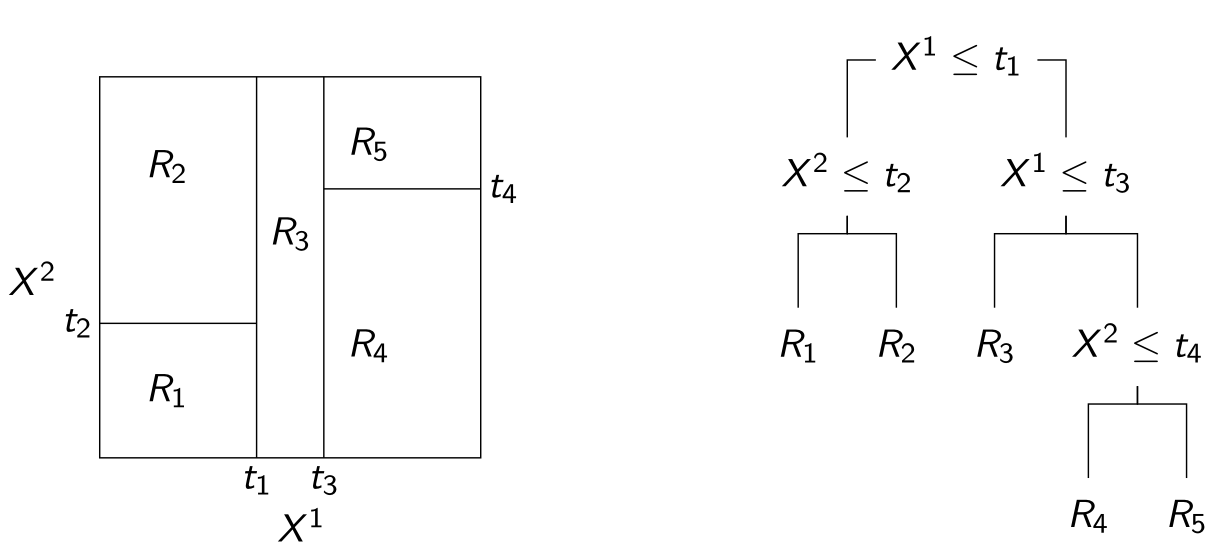
\includegraphics[width=0.8\linewidth]{images/03_methode/partition_cart}
	\caption{Schéma du partitionnement de l'espace des covariable par CART \cite{fischer2026}.}
	\label{fig:partitioncart}
\end{figure}

De manière plus formelle, on dispose d'un échantillon $\mathcal{D}_n = \{(X_1,Y_1),\dots,(X_n,Y_n)\}$ de couples indépendants et de même loi que $(X,Y)$, où $X = (X^{(1)},\dots,X^{(d)}) \in \mathbb{R}^d$ et $Y \in \mathbb{R}$. L'objectif est d'estimer la fonction de régression $f(x) = \mathbb{E}[Y \mid X = x]$. \\

\paragraph{Partitionnement et critère de coupure}
Un arbre partitionne récursivement l'espace des variables $\mathbb{R}^d$ en rectangles, chaque rectangle correspondant à un noeud de l'arbre. Soit $\mathcal{D}$ l'échantillon utilisé pour construire l'arbre, $R \subseteq \mathbb{R}^d$ un noeud et $n_R = \sum_{i}^n \mathds{1}_{\{X_i \in R\}}$ le nombre d'observations de $\mathcal{D}$ qui tombent dans $R$.\\

Une coupure est un couple $(j,t) \in \{1,\dots,d\} \times \mathbb{R}$, avec $j \in d$ la variable et $t \in \mathbb{R}$ le seuil de coupure. Elle partitionne le noeud $R$ en deux noeuds fils $R_1 (j,t)$ et $R_2(j,t)$ :
\[
R_1(j,t) = \{x \in R : x_j < t\}
\qquad\text{et}\qquad
R_2(j,t) = \{x \in R : x_j \ge t\},
\]
d'effectifs respectifs $n_1(j,t) = n_{R_1(j,t)}$ et $n_2(j,t) = n_{R_2(j,t)}$, avec $n_1(j,t) + n_2(j,t) = n_R$. 


On souhaite trouver une manière de partitionner les variables telle que les deux nouvelles régions $R_1 (j, t)$ et $R_2(j, t)$ issues de cette partition soient les plus homogènes possibles. Cela revient à, dans le cas de la régression, minimiser la variance de chaque noeud $R$ (critère d'impureté) :

\begin{equation}\label{eq:variance}
	V(R) = \frac{1}{n_R} \sum_{i : X_i \in R} \bigl(Y_i - \overline{Y}_R\bigr)^2
	\qquad\text{où}\qquad
	\overline{Y}_R = \frac{1}{n_R} \sum_{i : X_i \in R} Y_i .
\end{equation}

La qualité d'une coupure $(j,t)$ admissible est mesurée par la diminution d'impureté qu'elle produit, ou gain d'information (Information Gain, IG) :
\begin{equation}\label{eq:gain}
	\text{IG}_R(j,t) = V(R)
	- \frac{n_1(j,t)}{n_R}\, V\bigl(R_1(j,t)\bigr)
	- \frac{n_2(j,t)}{n_R}\, V\bigl(R_2(j,t)\bigr).
\end{equation}

Les variances des fils sont pondérées par la proportion d'observations qu'ils
contiennent, de sorte que $	\text{IG}_R(j,t) \ge 0$ (décomposition de la variance
totale en variances intra- et inter-groupes). La meilleure coupure parmi un
ensemble de variables candidates $\mathcal{M} \subseteq \{1,\dots,d\}$ est
\begin{equation}\label{eq:meilleure}
	(j^\star, t^\star) \in
	\text{argmax}_{j \in \mathcal{M},\; t \in \mathcal{T}_j(R)} 	\text{IG}_R(j,t).
\end{equation}

\paragraph{Prédiction d'un arbre}

Pour $x \in \mathbb{R}^d$, on note $R(x)$ la feuille de l'arbre $\hat f$ contenant $x$ et $n_{R(x)}$ le nombre de points de $\mathcal{D}_m$  qui y tombent. La prédiction de
l'arbre est la moyenne des réponses de cette feuille :
\begin{equation}
	\label{eq:arbre}
	\hat f(x) = \overline{Y}_{R(x)}
	= \frac{1}{n_{R(x)}}
	\sum_{(X_i,Y_i) \in \mathcal{D}_m} Y_i \, \mathds{1}_{\{X_i \in R(x)\}}
\end{equation}

\subsection{Forêt Aléatoire} 
\label{subsection:RF}
Une forêt aléatoire \cite{breiman2001} est une méthode de bagging consistant à tirer $B$ échantillons bootstrap à partir de $\mathcal{D}_n$, puis construire un arbre CART sur chacun d'eux et enfin agréger les prédictions des $B$ arbres. Les CART construits sont cependant légèremment différents : à chaque noeud, la meilleure coupure n'est pas cherchée parmi les $d$ variables, mais parmi un sous-ensemble de $p \le d$ variables tirées au hasard.

\paragraph{Construction de la forêt}
Pour $b = 1, \dots, B$, on tire avec remise un échantillon bootstrap $\mathcal{D}_m^{(b)}$ de taille $m$ dans $\mathcal{D}_n$, puis on construit un arbre $\hat f^{(b)}$ sur $\mathcal{D}_m^{(b)}$ par partitionnement récursif. À chaque noeud $R$, on tire uniformément et sans remise un ensemble $\mathcal{M} \subseteq \{1,\dots,d\}$ de $p$ variables, et on coupe $R$ selon la coupure $(j^\star, t^\star)$ définie par \eqref{eq:meilleure}. Le tirage de $\mathcal{M}$ est effectué indépendamment à chaque noeud. 

\paragraph{Prédiction de la forêt}
Pour chaque arbre $b \in [1, \ldots, B]$, la prédiction $\hat f^{(b)}(x)$ est donnée par \eqref{eq:arbre} (en remplaçant $\mathcal{D}_m$ par $\mathcal{D}_m^{(b)}$). La forêt prédit la moyenne des $B$ arbres :
\begin{equation}\label{eq:foret}
	\hat f_B(x) = \frac{1}{B} \sum_{b=1}^{B} \hat f^{(b)}(x).
\end{equation}

\paragraph{Hyperparamètres}
La construction de forêts aléatoires dépend donc de quatre hyperparamètres : 
\begin{itemize}
	\item $B$ le nombre d'arbres (\texttt{num.trees}),
	\item $m$ la taille des échantillons bootstrap (\texttt{sample.fraction}),
	\item $p$ le nombre de variables candidates pour chaque split (\texttt{mtry}),
	\item $n_{\min}$ l'effectif minimal des feuilles (\texttt{min.node.size})
\end{itemize}  
	
	
	
	
	
	
	
	
	
	
	
	
		



	
	\section{Protocole de validation croisée}
		\label{section:CV}
		\subsection{Prévention des fuites de données}
			Les données environnementales et biologiques présentent une structuration dépendante de la latitude : leurs propriétés statistiques varient donc selon la position dans l'espace. Les hypothèses de stationnarité d'ordre 1 (moyenne constante dans l'espace) et d'ordre 2 (structure de covariance invariante par translation, ne dépendant que de la distance entre points) ne sont donc pas respectées.
			
			De plus, lors des campagnes océanographiques, une onde acoustique est émise toutes les 3 à 4 secondes. La conséquence de cette proximité spatio-temporelle est la présence de pseudo-duplicatas dans le jeu de données. 
			
			Ces deux éléments, non-stationnarité spatiale et auto-corrélation, doivent être pris en compte lors de la construction du schéma de validation croisée, afin d'éviter toute fuite d'information entre les jeux d'entraînement et de validation (data leakage).
		\subsection{Validation croisée}
		
			% la description de la validation croisée est incomplète : il manque le pourquoi on fait ça !!
			La validation croisée est une méthode permettant consistant à diviser l'ensemble des données en $K$ sous-ensemble de taille à peu près identiques, appelés \textit{plis} (ou \textit{folds}). Un plis sert d'\textit{ensemble de validation} (ou \textit{ensemble test}) et les $K-1$ plis restants servent d'\textit{ensemble d'entraînement}. On obtient donc $K$ prédictions pour un même modèle. 
			
			Il existe différentes manières de sous-échantillonner les données pour construire les plis. Dans notre étude, nous avons testés différentes méthodes : validation croisée Monte-Carlo (Monte-Carlo Cross Validation, MC-CV) et la validation croisée par blocage spatio-temporel.
			\paragraph{Validation croisée Monte-Carlo (MC-CV)}
				Les analyses d'auto-correlation effectuée en section \ref{}
			\paragraph{Validation croisée par blocage spatio-temporel}
			
	\section{Ajustement des hyperparamètres}
	\section{Évaluation des performances}
		\subsection{Métriques et biais des prédictions}
	\section{Validation du modèle}
		\subsection{Sur-apprentissage et robustesse}
		\subsection{Recherche de raccourcis (shortcut learning)}
		\subsection{Domaine d'applicabilité}
	\section{Interprétation post-hoc}
		\subsection{Importance des variables (covariables corrélées)}
		\subsection{Analyse des résidus et suffisance des covariables}
	



















	\section{Schéma de validation}
	\section{Ajustement des hyperparamètres}
	\section{Validation}
	\subsection{validation des données}
	Le biais d'échantillonnage et le covariate shift portent sur les données : on peut les mesurer sans même avoir de modèle, en comparant les données d'entraînement à celles de la population cible ou de la production. C'est de la validation des données.
	\subsection{validation du protocole}
	La fuite de données porte sur le protocole : elle vient de la façon dont on a construit les variables, séparé les jeux d'entraînement et de test, ou choisi les informations disponibles au moment de prédire. La vérifier, c'est valider la conception de l'expérience.
	\subsection{validation du modèle}
	Valider un modèle, c'est établir qu'il est adapté à son usage prévu : que ses hypothèses tiennent, qu'il s'appuie sur des relations légitimes, qu'il reste fiable dans les conditions où il sera employé, et dans quel domaine il est applicable. Chercher à savoir à savoir si sa performance est fiable et si elle tiendra dans les conditions réelles.
	
	Le shortcut learning porte sur le modèle lui-même : il faut regarder ce qu'il a réellement appris, avec des outils d'interprétabilité ou des tests où l'on neutralise la variable suspecte. C'est de la validation du modèle au sens strict.
	
	Une fuite ou un biais d'échantillonnage dans les données est souvent ce qui rend possible un raccourci dans le modèle, et un décalage de distribution est ce qui fait apparaître ce raccourci en production.
	
	vérifier que le modèle n'overfit pas : robustesse au bruit
	vérifier que le modèle ne fais pas shortcut learning
	vérifier que le modèle est capable d'extrapoler 
	
	
	\section{Evaluation du modèle}
	vérifier que le modèle prédit de manière fiable et non biaisé
	
	\section{Interprétation post-hoc}
	\subsection{Importance des variables}
	\subsection{Source du biais} % mais ça en fait ca se fait avant sur la validation des données non ?
	\subsection{Suffisances des informations contenues par les covariables} % mais ça en fait ca se fait avant sur la validation des données non ?
	
	
	\clearpage
	\chapter{Résultats}
	\section{Structure et validation des données}   % décalages entre groupes, biais d'échantillonnage
	\section{Performances du modèle}                  % métriques en validation croisée par blocs, biais des prédictions
	\section{Validité du modèle}                      % raccourcis, robustesse, domaine d'applicabilité
	\section{Prédictions}                             % cartes, séries, sur le domaine validé
	\section{Interprétation}                          % importance des variables, effets partiels, résidus
	\clearpage
	\chapter{Discussion}
\section{L'échantillonage permet-il de répondre à la problématique ?}
- biais d'échantillonage et régions/années moins représentées => perf du modèle diminuées dans certaine régions
- distribution shift => un modèle n'est pas sufisant pour prédire toute la ROI (sauf peut être s'il apprend la causalité).
- valeurs manquantes MNAR et biais de sélection (couverture nuageuse)

\section{Les variables mesurées représentent elles correctement les construits ?}
incertitudes liées aux données :
- NASC et acoustique active
- classes de phyto a partir des pigments

\section{Prédiction ou explicabilité ?}

\section{Contrainte des modèles prédictifs}
- nécessité d'avoir une métrique rigoureuse d'évaluation des performances du modèle (CV blocage)
- nécessité de robustesse façe à l'extrapolation 
- en découle la nécessité de limiter le shortcut learning
- apprendre la causalité permet la robustesse face à extrapolation 

\section{Pertinence des forêts aléatoires}
- surapprentissage et RF : surapprentissage possible par profondeur des arbres
- diminution de la variance utile pour le trade-off biais-variance de la prédiction
- extrapolation difficile étant donné que RF est fonction continue par morceau 
- importance des variables sur echantillon OOB mais OOB est leaked/fortement correlé/biais d'echantillonage

\section{Mise en relation des résultats associatifs avec la théorie de causalité et hypothèses}
- liens entre mésoéchelle et distrib phyto 
- liens trophiques entre phyto et NTI mais délai
- liens avec importance des variables
- liens entre connaissance des distribs de euphausiaces et prédictions
- liens entre connaissance inversion 18/38 et observations + distributions des poissons 38 et prédictions

\section{Domaine d'applicabilité du modèles et précautions d'interprétations}

\section{perspectives}
	\clearpage
	\listoffigures
	\listoftables
	
	\printbibliography
\end{document}